% !TeX encoding = UTF-8
% !TeX program = pdflatex
% !BIB program = biber

% Template Revision:
% Rev. C3 -- 2022-03-07 -- Ali Varli
% Rev. C2 -- 2021-05-11 -- Ali Varli
% Rev. C1 -- 2021-03-22 -- Ali Varli
% Rev. B1 -- 2019-11-05 -- Ali Varli

%% HINWEISE:
%% MAIN.tex ist die Hauptdatei. Hier sind sämtliche Pakete eingebunden und die allgemeine Struktur ist hier festgelegt. Im Allgemeinen müssen hier keine Änderungen vorgenommen werden.
%% In der eingebundenen Datei config.tex müssen Änderungen vorgenommen werden, die in der Datei näher erläutert sind.
%% Das Deckblatt wird mit der Datei cover/coversheet.tex eingebunden. Hier sollten keine Änderungen vorgenommen werden.
%% Für Text im Vorspann (vor der Inhaltsangabe, z.B. für Vorwort, Abstract etc.) ist die Datei frontmatter.tex vorgesehen.
%% Für den Hauptteil ist die Datei mainmatter.tex vorgesehen.
%% Das Literaturverzeichnis ist die eingebundene Datei literature.bib.
%% Die erzeugt Ausgabe ist PDF/A-1B-kompatibel. Bei eingebundenen Dateien (PDFs, PNGs etc.) sollte darauf geachtet werden, dass diese ebenfalls PDF/A-kompatibel sind (PNGs mit transparentem Hintergrund sind es z.B. nicht).
%% Für Verbesserungsvorschläge bin ich gerne offen.
%% Viel Erfolg :). Linz, im Oktober 2019, Ali Varli, a_v@gmx.net.

%% PLEASE NOTE:
%% MAIN.tex is the main file. All packages are pooled here and the general structure is defined here. In general, no changes need to be made here.
%% Changes must be made in the included file config.tex. Detailed information is in the file.
%% The cover page is included with the file cover/coversheet.tex. No changes should be made here.
%% The file frontmatter.tex is provided for text in the lead text (before the summary, i.e. for the foreword, abstract, etc.).
%% The file mainmatter.tex is intended for the main part.
%% The bibliography is the included file literature.bib.
%% The produced output is PDF/A-1B-compliant. Embedded files (PDFs, PNGs etc.) must be also PDF/A-compliant (e.g. PNGs with transparent backgrounds are not PDF/A-compliant).
%% I am open to suggestions for improvement.
%% Good luck :-). Linz, October 2019, Ali Varli, a_v@gmx.net.


\NeedsTeXFormat{LaTeX2e}[2019-10-01]
\documentclass[%
	a4paper,
	11pt,
	BCOR=10mm,
	DIV=12,
	headinclude,
	headheight=16mm,
	oneside,
	onecolumn,
	openany,
	parskip=half,
	% appendixprefix,
	% toc=flat,
	% chapterentrydots=true,
	table,
	fleqn,
	% draft
]{scrbook}

\usepackage[utf8]{inputenc}

% !TeX encoding = UTF-8
% !TeX root = MAIN.tex

\newif\ifeng
%% HINWEISE: Hier müssen folgende Einstellungen vorgenommen werden:
%% PLEASE NOTE: Select your settings here:

%% Sprache: Falls die Dokumentensprache Deutsch ist, \engtrue mit einem %-Zeichen davor auskommentieren:
%% Language: If the document language is German, comment \engtrue with a % sign in front:
\engtrue

%% Hier den Namen des Autors eingeben:
%% Enter the author’s name here:
\def\author{Alexander Krauck}

%% Hier Informationen für den rechten Block unter dem JKU-Logo eingeben, wobei die Elemente mit einem Buchstaben jeweils für die Beschreibung und mit Doppelbuchstaben für den Inhalt sind.
%% Anzuführen bei Masterarbeit: Eingereicht von, Anfegertigt am, BeurteilerIn, Mitbetreuung.
%% Anzuführen bei Dissertation: Eingereicht von, Anfegertigt am, ErstbeurteilerIn, ZweitbeurteilerIn, Mitbetreuung.
%% Anzuführen bei strukturiertem Doktorat: Eingereicht von, Angefertigt am, ErstbetreuerIn, ZweitbetreuerIn, Mitbetreuung.
%%
%% Enter information here for the right block under the JKU logo, whereby the elements should have one letter for the heading and double letters for content.
%% To be given for master thesis: Author, Submission, Thesis Supervisor, Assistant Thesis Supervisor.
%% To be given for doctoral thesis: Author, Submission, First Supervisor, Second Supervisor, Assistant Thesis Supervisor.
\def\elementA{Author / Eingereicht von}
\def\elementAA{\textbf{\author} \\ Matriculation number / Matrikelnummer \\ \textbf{K11904235}}

\def\elementB{Submission / Angefertigt am}
\def\elementBB{\textbf{Institute of Machine Learning}}

\def\elementC{Thesis Supervisor / First Supervisor / BeurteilerIn / ErstbeurteilerIn / ErstbetreuerIn}
\def\elementCC{DI~Dr.\@ \textbf{Name}}

\def\elementD{Second Supervisor / ZweitbeurteilerIn / ZweitbetreuerIn}
\def\elementDD{\textbf{Name}}

\def\elementE{Assistant Thesis Supervisor / Mitbetreuung}
\def\elementEE{\textbf{Name}}

%% Hier Datum eingeben (Monat der Abgabe im Prüfungs- und Anerkennungsservice):
%% Enter the date (Month and year of submission to Examination and Recognition Services):
\def\date{Mai 2024}

%% Hier Ort eingeben:
%% Enter the location:
\def\place{Linz}

%% Hier Titel eingeben; steht über dem K:
%% Enter the title; it appears above the K:
\def\title{Conditional Density Estimation and Conformal Prediction are Equivalent Tasks in Regression}

%% Hier den Typ der Arbeit eingeben (0: Keine Arbeit, 1: Bachelorarbeit, 2: Masterarbeit, 3: Dissertation, 4: Diplomarbeit):
%% Enter the type of paper here (0: Not Thesis, 1: Bachelor’s Thesis, 2: Master’s Thesis, 3: Dissertation, 4: Diploma Degree Thesis):
\def\type{2}

%% Hier ggf. Untertitel eingeben; stehen unter dem K (nur bei 0):
%% If necessary, enter a subtitle here; below the K (only for 0):
\def\subtitle{}

%% Hier den angestrebten akademischen Grad eingeben:
%% Enter the desired academic degree here:
\def\acadDegree{Master of Science}

%% Hier die Studienrichtung eingeben:
%% Enter the major here:
\def\study{Artificial Intelligence}

%% Hier die Metadaten für das PDF eingeben (mehrere Autoren und Keywords durch \sep trennen):
%% Enter metadata for the PDF here (seperate multiple authors and keywords by \sep):
\begin{filecontents*}[overwrite]{\jobname.xmpdata}
\Title{Test\title}
\Author{Alexander Krauck\author}
\Subject{}
\Keywords{}
\Language{en-US}
\Publisher{}
\end{filecontents*}

\usepackage[a-1b]{pdfx}[2019-02-27]
\usepackage[T1]{fontenc}
\usepackage{helvet,mathpazo}
\usepackage{microtype}
\ifeng
	\usepackage[naustrian,english]{babel}
\else
	\usepackage[english,naustrian]{babel}
\fi
\usepackage[absolute]{textpos}
\usepackage{amsmath,siunitx}
\usepackage[%
	%backend=biber,
	style=authoryear, % authoryear
    %citestyle=authoryearbrack
	%bibstyle=authoryear, % authoryear
	%citestyle=authoryear-comp, % authoryear
	% maxcitenames=2,
	%sorting=none, %nty
	%backref=true,
	%backrefstyle=none,
    %natbib=true
]{biblatex}
\usepackage{csquotes}
\usepackage{lastpage,scrlayer-scrpage}
\usepackage[onehalfspacing]{setspace}
\usepackage{booktabs,colortbl,xcolor}
\usepackage{graphicx,wrapfig}
\usepackage[section]{placeins} %\FloatBarrier
\usepackage{float} %[H]
\usepackage{enumitem}
\usepackage{subfiles}
\usepackage{scrhack}
%\usepackage[colorlinks=true, allcolors=blue]{hyperref}%mine


% \setcounter{tocdepth}{3} %subsubsection
% \setcounter{secnumdepth}{3}

\newpairofpagestyles[scrheadings]{jku}{%
	\clearpairofpagestyles
	\ifeng
		\ohead*{\includegraphics[width=3cm]{cover/jkuen}}
	\else
		\ohead*{\includegraphics[width=3cm]{cover/jkude}}
	\fi
	\ifoot*{\date}
	\cfoot*{\author}
	\ofoot*{\pagemark/\pageref{LastPage}}	
	\setkomafont{pageheadfoot}{\sffamily\scriptsize}
	\setkomafont{pagenumber}{\sffamily\scriptsize}
}

\hypersetup{%
	bookmarksnumbered=true,
	pdfborder={0 0 0},
}

\tolerance=300
\clubpenalty=10000
\widowpenalty=10000
\displaywidowpenalty=10000

%------------------------------------------------------
%My own config stuffs
%\setcitestyle{authoryear}
\usepackage{amsthm}
\usepackage{amssymb}
\usepackage{multicol}
\usepackage{svg}
\usepackage{subfig}
%\usepackage[square,numbers]{natbib}
\usepackage{stackengine}
\usepackage[english]{babel}
\usepackage{datetime}
\usepackage{dsfont}
\usepackage{dcolumn}
\usepackage{algorithm} % for pseudocode
\usepackage{algorithmic} % for pseudocode
\usepackage{xargs} % for commands with multiple arguments
%\usepackage{subcaption}
\usepackage{subfig}
\usepackage{mathrsfs}

\newcolumntype{d}[1]{D{.}{.}{#1}}

%\DeclareCiteCommand{\cite}[\mkbibbrackets]
%  {\usebibmacro{prenote}}
%  {\usebibmacro{citeindex}%
%   \usebibmacro{author}%
%   \setunit{\labelnamepunct}\newblock
%  \usebibmacro{date}}
%  {\multicitedelim}
%  {\usebibmacro{postnote}}


\AtEveryCite{%
  \let\parentext=\parentexttrack%
  \let\bibopenparen=\bibopenbracket%
  \let\bibcloseparen=\bibclosebracket}

\usepackage{letltxmacro}\LetLtxMacro{\cite}{\parencite}
\renewcommand*{\nameyeardelim}{\addcomma\space} 
\DeclareCiteCommand{\cite}[\mkbibparens]
  {\usebibmacro{prenote}}
  {\usebibmacro{citeindex}%
   \printtext[bibhyperref]{\color{orange}\usebibmacro{cite}}}
  {\multicitedelim}
  {\usebibmacro{postnote}}

\DeclareCiteCommand*{\cite}[\mkbibparens]
  {\usebibmacro{prenote}}
  {\usebibmacro{citeindex}%
   \printtext[bibhyperref]{\color{orange}\usebibmacro{citeyear}}}
  {\multicitedelim}
  {\usebibmacro{postnote}}

\hypersetup{
    citecolor=orange,
    linkcolor=green,
    urlcolor=blue % Change 'blue' to whatever color you prefer for URLs
}



\newcommand\pef[1]{\hyperref[#1]{\color{green}Section~\ref{#1}}}
\newcommand\fef[1]{\hyperref[#1]{\color{green}Figure~\ref{#1}}}
\newcommand\tef[1]{\hyperref[#1]{\color{green}Table~\ref{#1}}}
\newcommand\eef[1]{\hyperref[#1]{\color{green}Equation~\ref{#1}}}

\newcommandx{\sref}[2][1=]{\hyperref[#2]{\color{green}#1~\ref{#2}}}


\DeclareMathOperator*{\argmin}{arg\,min}
\DeclareMathOperator*{\argmax}{arg\,max}

\newtheorem{theorem}{Theorem}[section]
\newtheorem{lemma}[theorem]{Lemma}
\theoremstyle{definition}
\newtheorem{definition}{Definition}[section]
%----------------------------------------------

% \addtocontents{toc}{\protect\enlargethispage{2\normalbaselineskip}}
% \addtocontents{lof}{\protect\enlargethispage{2\normalbaselineskip}}
% \addtocontents{lot}{\protect\enlargethispage{2\normalbaselineskip}}

\addtokomafont{caption}{\small}
\setkomafont{captionlabel}{\small\sffamily\bfseries}

%% Literaturdatenbank / Bibliography:
\addbibresource{references.bib}

%% Seitenstil / Pagestyle:
%\pagestyle{jku}

%
%%
%%%%
%%%%%%%%
%%%%%%%%%%%%%%%%
\begin{document}
%%%%%%%%%%%%%%%%

\begin{titlepage}
	\setcounter{page}{0}
	\include{cover/coversheet}
\end{titlepage}


%%%%%%%%%%%%
\frontmatter

% !TeX encoding = UTF-8
% !TeX root = MAIN.tex

{%
	\selectlanguage{naustrian}
	\chapter*{Kurzfassung}
	
	Kurzfassung auf Deutsch.
}

{%
	\selectlanguage{english}
	\chapter*{Abstract}
	
	Abstract in English.
}

\begin{singlespace}
	\tableofcontents
	\listoffigures 
	\listoftables
\end{singlespace}


%%%%%%%%%%%
\mainmatter

% !ht
% !TeX root = MAIN.tex

\chapter{Introduction}\label{chap:introduction}

Machine Learning (ML) models that can not only estimate single targets accurately, but that are capable of estimating distributional information as well as uncertainty are becoming exceedendly important~\cite{hullermeier_aleatoric_2021, gawlikowski2023survey}. The reason therefore is, that most modern ML techniques are mostly black box models that have little intuitive reason behind their predictions but often act on abstract latent representations, especially in the case of Artificial Neural Networks (NN). With a strong focus on regression tasks, in this work we aim to develop a novel understanding of uncertainty estimating methods, where in particular we show that we can combine ideas from multiple different task-types. We show that Conditional Density Estimation (CDE), Conformal Prediction (CP) and Quantile Regression (QR) are fundamentally the same task since they all require to model parts of the conditional probability density function (PDF). Moreover, we develop a novel way to perceive the maximum log likelihood (MLL) objective function, where we show that it is equivalent to the objective function of CP, as we define it. This allows us to split the MLL objective into a constrainted optimization problem, where we intuitively minimize the size of the peaks (we make them as narrow as possible) with the constraint that we maintain calibration. Finally, we aim to introduce a novel way of perceiving epistemic uncertainty in CDE.\@ All details to the theoretical concepts and novel insights are detailed in \pef{chap:theoretical}.

Before we go into the details of the theoretical background, we want to give a brief overview of the motivation, the exact research questions that we aim to answer in this work and a summary of the contributions. In particular, the practical implications and applications of this work are first discussed below in \pef{sec:background}. Even though this work is not centered around a particular practical application but is more at home in the theoretical part of machine learning the author of this work belives that a motivation in the practical domain is very important to make the work more accessible and to show the relevance of the work. In particular, we aim to show that the methods proposed in this work can be applied to a broad range of practical tasks and that they can have a significant positive impact on the performance of machine learning models in those tasks.

\section{Background}\label{sec:background}

Mostly in risk-sensitive practical domains like finance and life science uncertainty estimation is crucial~\cite{abdar2021review, xia2020uncertainty, ghesu2021quantifying, mashrur2020machine}. Therefore there exist two fundamental approaches to perceive uncertainty. First, there is the uncertainty that is inherent in the data, which means that for a give input, there are multiple possible outputs which are plausible, which also can not be reduced. This is called aleatoric uncertainty and it is the main task of CDE and CP to estimate this kind of uncertainty. Secondly, and less researched in the domain of regression, there is the uncertainty of the model, which could occur if the model is shown a sample that it can not generalize to, based on the training data it was trained on. This uncertainty is termed epistemic uncertainty. In this work we argue that in order to make reliable and informed decisions in high risk tasks, it is crucial to have methods to estimate both kinds of uncertainty, however, most recent works in regression tasks exclusively focus on estimating aleatoric uncertainty~\cite{romano2019conformalized, sesia2020comparison, angelopoulos2021gentle,chernozhukov2021distributional,sesia2021conformal, oliveira2022split, romano2022conformal, izbicki2022cd, gupta2022nested, auer2024conformal}. In particular, methods like CDE, CP and QR can only directly estimate the aleatoric uncertainty, which is also the reason why epistemic uncertainty has been out of focus. However, in this work we argue that a type of epistemic uncertainty is already unknowingly being induced into models in many cases, that is with calibration.

\subsection{Uncertainty in Finance}\label{sec:intro_finance}

\subsubsection{Energy Price Prediction}

A practical task that we particularly focus on in this work is an energy price prediction task, in cooperation with Voestalpine AG which provided us with the dataset for the scope of this Master's Thesis, where we attempt to estimate the distribution of the imbalance energy price\footnote{For precise details on this quantity we refer to \url{https://markttransparenz.apg.at/en/markt/Markttransparenz/Netzregelung/Ausgleichsenergiepreise}} of Austria given multiple descriptive input variables/features. In particular, the imbalance energy price we aim to predict is unknown at the time of consumption/production and is only much later revealed.

If an entity on the energy market wants to buy or sell electricity at a certain time, this entity does indicate how much electricity it wants to buy or sell for the dayahead price which is known. Hoever, if this entity produces/consumes more energy than agreed on, the energy imbalance price holds for this over-/underestimation, but this price is only known after the fact and heavily depends on what other entities on the market did. In particular, the imbalance energy price is a very volatile price, making it a relevant use case for uncertainty estimation since it can impact the decision if electricity should be bought or produced at a given time.

\subsubsection{Stock Price Prediction}
In more traditional finance tasks, we mostly try to predict price-trends of assets like stocks~\cite{singh2017stock}, currencies~\cite{hassanpour2023evaluation}, cryptocurrencies~\cite{alessandretti2018anticipating} and other equities. Those predictions are then used either for assisted decision making of analysists or for automated and potentially high frequency trading. Especially when making decisions with high stakes it is crucial to know exactly the risk that is taken with a certain decision, ideally with certain gurantees. For example, it might be essential not to loose more than a specified amount of money with a trading decision with a certain probabilistic confidence level. A known quantity in trading is the Value at Risk (VaR) as introduced by~\cite{jorion2007value}, which is the maximum amount of money that can be lost with a certain confidence level.

\subsection{Uncertainty in Healthcare and Life Science}

In life science uncertainty aware ML methods have also been of increasing interest~\cite{loftus2022uncertainty, lambert2024trustworthy}. Often it is of relevance to estimate some regression targets like from personalized drug dosage prediction~\cite{wu2023application}, amniotic fluid volume prediction~\cite{csillag2023amnioml}, tumor size quantification~\cite{prasad2023tumor}, time-to-event prediction~\cite{kvamme2019time, sloma2021empirical}. It is crucial for those tasks to not only know the average outcome, but to also be able to see if there are small probability events that could still happen with some plausible probabilitly. For example, if we predict the size of the tumor of a patient, the main probability density peak might be at a certain size, but it might be possible that there is another smaller peak at a much larger size which could lead to a more urgent tratment strategy. In this case, it is crucial to know the full distribution of the target variable and not only the mean. For similar reasons the epistemic uncertainty is also extremely relevant there. The model might not be able to generalize to a certain patient, which could lead to a completely random prediction and thus to a horrible decision if the doctor is not informed about the uncertainty of the model.

\section{Related Work and Motivation}\label{sec:motivation}

Many different related works about CDE~\cite{bishop1994mixture, rothfuss2019conditional, trippe2018conditional, rothfuss2019noise, ambrogioni2017kernel}, CP~\cite{izbicki2022cd, chernozhukov2021distributional,romano2019conformalized, Papadopoulos08, angelopoulos2021gentle}, QR~\cite{chung2020beyond} aswell as uncertainty estimation in general~\cite{gal_dropout_2016, hullermeier_aleatoric_2021, abdar2021review, klotz2021uncertainty} have been published in recent years. Most of those methods essentially attempt to model certain parts of the uncertainty of target variables given descriptive feature variables. Moreover, there exist works that observe that certain concepts can be transferred from one domain of uncertainty estimation to another~\cite{chernozhukov2021distributional}.
We will here provide a brief overview of CDE, CP and QR with focus on the recent works on those topics and a overview over practical methods that are used for those tasks currently. Only later in \pef{chap:theoretical} we will give precise definitions of those tasks since there we also have established the notation.

\subsection{Recent Works in CP}

Initially CP was done by simply scaling a homoscedastic interval around the mean estimator of the data~\cite{lei2018distribution}. However, many limitations come with this approach and so other approaches that take into account heteroscedasticity have come forth, in particular a very prominent method for a significance level of $2 \alpha$ to estimate the quantiles at $\alpha$ and $1 - \alpha$~\cite{romano2019conformalized}. The most recent works have gone away from this also and now primarely focus on predicting the shortest CP intervals~\cite{sesia2021conformal,chernozhukov2021distributional,izbicki2022cd} in expectation. In particular, therefore often distributional information is required in order to effectively obtain the shortest CP intervals which has a strong relation to CDE quite obviously. However, no previous work goes into the details of the exact relationship between CP and CDE.\@

\subsection{Recent Works in CDE}

The most simplistic way of estimating conditional PDFs is just estimating the mean and inferring the optimal homoscedastic variance from the data which also aligns with the assumption of a Gaussian error model in the case of the mean squared error. The next step would be to estimate the variance also for each sample to obtain heteroscedasticity. However, since this still comes with major limitations a very fundamental work has been by~\cite{bishop1994mixture} where they propose to model the conditional PDF as a mixture of simple distributions like Gaussians/Laplacians. This method is called Mixture Density Networks (MDNs) and is still the most prominent method for CDE.\@ However, it is also very prone to overfitting and so other methods like Kernel Mixture Networks (KMNs) have been proposed~\cite{ambrogioni2017kernel}. In particular, one of the most recent works in CDE has been done by~\cite{rothfuss2019noise} where they propose a method to mitigate the overfitting problem of MDNs by adding noise to the input data. However, no previous work goes into the details of the exact relationship between CDE and CP.\@ Additionally some other recent works on CDE like Normalizing Flow Networks~\cite{trippe2018conditional} exist, however this method still can not outperform MDNs or KMNs in practice.

\subsection{Recent Works in QR}

QR is was already explored in the 70s and 80s~\cite{koenker1978regression} and has since then been a very prominent method for estimating quantiles of the target variable by using the Pinball Loss. Moreover, more recent works in QR exist by~\cite{chung2020beyond} where they establish some connection between QR, CP and CDE already, which will be discussed in more detail in the theoretical part of this work.

\subsection{Recent Works in Uncertainty Techniques}

In recent years the possibly most prominent topic of uncertainty in machine learning has been the estimation of epistemic uncertainty~\cite{barber1998ensemble, neal2012bayesian, gal_dropout_2016,schweighofer2023quantification, gawlikowski2023survey} where the main task is to estimate the model's confidence, that it's predictions are accurate, given an unseen sample. This is not to be confused with the conditional PDF produced by CDE methods, which only models a different type of uncertainty as discussed in more detail in \pef{sec:uncertainty_calibration}.

%maybe add a practical related work thing where I introduce the models that exist like MDN, KMN, etc. 
\subsection{Practial Methods}
Methods that are currently used for the purpose of CDE, CP and QR are manifold. We will give an overview over the most prominent and well performing methods in the following.

\paragraph{MDNs} are probably the most prominent method for CDE by~\cite{bishop1994mixture}. They are based on the idea of modeling the conditional PDF as a mixture of simple distributions e.g. Gaussians or Laplacians. In MDNs a NN is used to predict the parameters of the mixture components. In the case of Gaussians, the parameters are the mean, variance and the component weights. The mixture components are then combined to form the full conditional PDF.\@ MDNs are very expressive and can model multimodal distributions very well. However, they are also very prone to overfitting, but recent methods like~\cite{rothfuss2019noise} aim to mitigate this problem effectively. MDNs are usually optimized using the negative log likelihood loss function.

\paragraph{KMNs} are a more recent development by~\cite{ambrogioni2017kernel}. They are based on the idea of selecting kernel centers from the training samples by clustering techniques like K-Means. The kernel centers are then used to form a kernel mixture model, where the kernel centers are the mixture components. The kernel mixture model is then used to estimate the conditional PDF.\@ KMNs are less expressive than MDNs, but they are also less prone to overfitting and can be more robust in practice. Conceptually they are similar to MDNs where the mixture components are formed by the kernel centers. KMNs are also optimized using the negative log likelihood loss function.

\paragraph{Multiple Quantile Regression (MQR)} is a method that is based on the idea of estimating multiple quantiles of the target variable. In particular, when doing simple QR we may only have a single quantile, which can be choosen aribtrarily. However, in MQR we estimate multiple quantiles at once. This can be done by using a single NN that outputs multiple quantiles at once or by using multiple NNs that each output a single quantile. MQR has been used to accomplish CP in the past by~\cite{sesia2021conformal} very successfully. In particular, for CP it is the current state-of-the-art (SOTA) method. MQR is optimized by using the Pinball Loss objective function, which is a quantile regression specific loss function.

In conclusion the topic of uncertainty estimation is rapidly growing recently and in works like~\cite{chernozhukov2021distributional} implicitly it has been shown that there is a connection between CP, CDE and QR.\@ However, no previous work has gone into the details of the exact relationship between those methods. Moreover, the conceptual position of epistemic uncertainty in the context of CP, CDE and QR is not well understood.

\section{Research Questions}\label{sec:questions}

Within this work we aim to answer two main questions. The first and most essential question is how exactly CP, CDE and QR are related. As noted previous methods already implicitly show there must be a connection~\cite{sesia2021conformal,chernozhukov2021distributional,chung2020beyond} but lack a precise framwork for their practical application.

Based on this main question other questions arise:

\begin{itemize}
    \item Can we develop a general framework on which basis techniques from one of those methods can be transferred to another method?
    \item What optimization strategy should we choose or which ones can we even choose. CDE mostly relies on the MLL objective function, while CP often relies on the pinball loss. Based on the insights we gain in this work, we want to gain more insight into this question.
    \item Based on the relation between those methods, can we gain more insight into the often made claim that CP and QR are fundamentally distribution free methods? If they are related with CDE, which is often considered a distribution based method, then how can they be distribution free?
\end{itemize}

The second main question is how uncertainties, in particular aleatoric and epistemic uncertainties, are present in those uncertainty methods and in particular what kinds of in the sense of~\cite{hullermeier_aleatoric_2021}. In particular, one major observation is that even on the train data often uncertainty models are not calibrated, but it has not really been extensively treated yet why this is. We often just calibrate CP on the calibration set as in~\cite{sesia2021conformal} but what assumptions are we making when recalibrating. This is also rooted in the realization that in the context of CP, being calibrated alone is actually a trivial task since we can just calibrate on the marginal distribution of the targets.

\section{Contributions}\label{sec:contributions}

The main contributions of this work are as follows:

\begin{itemize}
    \item We show that CDE, CP and QR all have the same goal, that is they all restric the set of possible conditional PDFs, and that all concepts of one task-domain can fully be transferred to the other one.
    \item We propose a novel way to perceive the MLL objective function, where we show that it is equivalent to the objective function of CP, as we define it. This allows us to split the MLL objective into a constrainted optimization problem, where we intuitively minimize the size of the peaks (we make them as narrow as possible) with the constraint that we maintain calibration.
    \item We show that it might improve CP intervals if we can use properties of inductive biases provided by e.g.\ a mixture of Gaussians estimtated by using MDNs.
    \item We offer a novel way to estimate epistemic uncertainty in CDE and CP methods, where we show that calibration as often done in CP, actually infuses epistemic uncertainty into the modeled PDF that describes only aleatoric uncertainty.
    \item Finally we empirically verify our insights on multiple benchmarks and show that our method is competitive with SOTA methods and that it can be applied to a wide variety of tasks. Thereby, we also provide a general overview of hyperparameters that are generally a good choice for CDE,CP and QR tasks. In particular we also propose few new hyperparameters and analyze their impact.
\end{itemize}

\section{Structure of the Work}\label{sec:structure}

First, in \pef{chap:theoretical} we give a thorough introduction into CP, CDE and QR and show they are fundamentally the same task. Moreover, we show how we can infer CP from CDE and how we can estimate epistemic uncertainty in CDE and CP methods. In \pef{chap:empirical_study} we show how our insights can be applied to a wide variety of tasks and how they improve the performance of CDE, QR and CP methods. Finally, in \pef{chap:conclusion} we summarize our insights and give an outlook on future work.

Notably, novel contributions and existing concepts are intervoven in the theoretical part of this work, as tearing them appart would heavily reduce the smooth line of argumentation present in this work and make notation much harder. In particular, this is because we will generalize existing concepts with new interpretations. However, we will always explicitly state if a concept is novel or if it is based on existing concepts. (Sub-) sections that contain a core contribution are marked with a star like \textbf{Section*}. However, also other section contain novelties that are not marked with a star; We made sure to always explicitly state if a concept is novel. It should be quite clear from the context if a concept is novel or not.

\chapter{Theoretical Analysis}\label{chap:theoretical}

\section{Preliminaries}\label{sec:preliminaries}

In the rest of this work we will unless stated otherwise always be assuming a machine learning task where samples have the assumption of independently and identically distribution (IID). Moreover, for the theoretical part of this paper, we also assume that we have unlimited samples unless stated otherwise which is necessary to make certain theoretical statements and in particular with limted data those statements all hold asymptotically.

Thus, unless stated otherwise, let $\left(\Omega, \mathcal{F}, \mathbb{P}\right)$ be a probability space. Furthermore, let $\mathbf{Z} = (\mathbf{X}, \mathbf{Y})$ random variables and $\mathbf{Y}: \Omega \to \mathbb{R}^m$ where each pair represents one sample. Moreover, let all $(\mathbf{X}, \mathbf{Y})$ be IID.\@

However, in many proofs in this paper we will not require the use of the probability space explicitly since we often just integrate over the whole sample space $\mathbb{R}^{n+m}$.

The task of the ML methods discussed here is always to predict some property, like the conditional PDF, about the target variable $\mathbf{Y}$ given the features $\mathbf{X}$. In the more practical case we only have access to some samples of $\mathbf{Z}$, which is the observed data set $\mathcal{D} = \left\{\left(\mathbf{X}_i, \mathbf{Y}_i\right)\right\}_{i\in I_{\mathcal{D}}}$, with $|I_{\mathcal{D}}| < \infty$.

Moreover, any model that we discuss here, regardless if it is CDE, CP or QR, will be parameterized by some parameters $\theta \in \Theta$ where $\Theta$ is the parameter space. Furthermore, we will always in this work make the assumption that the model class class can perfectly model the true model, which seems like a strong assumption, but considering that we focus on model classes that either can be tweaked to be very expressive or NN's that even are universal function approximators~\cite{HORNIK1989359}, this assumption is not unreasonably strong. The optimal parameter set is indicated by $\theta^*$.

For the above definitions of the probability space and random variables, the corresponding PDF of and event $\mathbf{z} = (\mathbf{x}, \mathbf{y}) \sim (\mathbf{X}, \mathbf{Y})$ is defined by
\begin{equation}\label{eq:pdf}
    p(\mathbf{x}, \mathbf{y}):=\frac{d^2 \mathbb{P}(\mathbf{X} \leq
        \mathbf{x}, \mathbf{Y} \leq \mathbf{y})}{d \mathbf{x} d \mathbf{y}}
\end{equation}
for $\mathbf{x} \in \mathbb{R}^n$, $\mathbf{y}\in\mathbb{R}^m$. It is left as a hint to the reader that $\mathbb{P}(\mathbf{X} \leq
    \mathbf{x}, \mathbf{Y} \leq \mathbf{y})$ in \eef{eq:pdf} is the cumulative distribution function (CDF). The marginal and conditional PDFs can then be found by integrating out and normalizing with the marginal respectively.

Finally in order to analytically show certain results we require some standard assumptions of the underlying conditional PDF $p(\cdot\mid \mathbf{x})$ which hold $\forall \mathbf{x}\in \mathbb{R}^n$.

\begin{definition}[Standard Assumptions]\label{def:assumptions} %TODO move that above to basic notations etc
    Our standard assumptions that we will impose on the true conditional PDFs that we aim to predict:
    \begin{enumerate}

        \item The PDF $p$ is continously differentiable almost everywhere (a.e.)
        \item $\forall b\in\mathbb{R}^+: \mathbb{P}(p(\mathbf{Y}) = b\mid \mathbf{x}) = \lambda(p(\mathbf{Y}) = b \mid \mathbf{x}) = 0$ (There are no plateaus in the PDF)
        \item $p > 0$ a.e.
    \end{enumerate}
\end{definition}

Those assumptions are weak in practice since we can approximate any PDF that does not fullfill those assumptions with a PDF that does fullfill those assumptions arbitrary well. We refer to~\cite{klenke2013probability} for a formal argument why this is true. Moreover, note that \sref[Assumption]{def:assumptions} imply that the quantile function $Q(\cdot)$ is well defined for all $q\in[0,1]$ since the corresponding CDF is necessarily strictly increasing which is left without proof but the intuition follows from \sref[Lemma]{lem:continuity}.

In the following we will first detail the three main uncertainty centric tasks already introduced in \pef{sec:motivation}, namely CDE in \pef{sec:cde}, CP in \pef{sec:cp} and QE in \pef{sec:qr}. We will then show how those tasks are fundamentally the same in \pef{sec:cp_sub_cde}, that optimizing the MLL objective function is equivalent to optimizing the CP objective function as we define it in \pef{sec:optimal_cp} and finally a rigorous examination of recalibration where we show that it infuses epistemic uncertainty into the modeled conditional PDF that describes only aleatoric uncertainty in \pef{sec:calibration} and \pef{sec:uncertainty_calibration}. It given as a recommendation to the reader to read the sections in order as certain essential concepts that are introduced in the first sections are used in the later sections.

\section{Conditional Density Estimation}\label{sec:cde}

The goal of CDE methods is to estimate the conditional PDF $p(\mathbf{y}\mid \mathbf{x})$ of samples $(\mathbf{x}, \mathbf{y}) \sim \mathbf{Z}$. The objective function used for CDE is usually likelihood function, which is given by $p(\mathbf{y}\mid \mathbf{x})$ for one sample and $\mathbb{E}_{\Omega}\left[\log p(\mathbf{Y} \mid \mathbf{X})\right]$ generally, where we take the logarithm of the likelihood function and thereafter can take the expectation over the whole sample space, which is valid since the logarithm is a strictly monotonous function.

\subsection{Smoothness Assumptions}\label{sec:smoothness}
In the context of CDE, it is crucial to see that we have an incredible amount of freedom in the output space. In particular, much more freedom than in the context of a usual regression task. This is because we do not only need to predict the mean of the target variable, but we need to predict the full distribution of the target variable with the nuance that we can not even expect to see two different targets for the same feature sets in many cases.

However, as we usually in the context of ML like to obtain a model that can generalize, we need to make smoothness assumptions in the context of CDE, as without them it is easy to define the optimal model as the delta function at the observed data points which is not a useful model as it will not generalize to new data points as will be discussed in more detail in \pef{sec:connection_model_producing}.

As we can see in the work of~\cite{rothfuss2019noise} the objective function of the model equals

\begin{equation}
    \arg \max _{\theta \in \Theta} \sum_{i=1}^n \log
    \hat{f}_\theta\left(x_i\right)=\arg \min _{\theta \in \Theta}
    \mathcal{D}_{K
        L}\left(p_{\mathcal{D}} \| \hat{f}_\theta\right)
    \label{eq:kl_divergence_mll}
\end{equation}

where $p_{\mathcal{D}}$ is the delta distribution with peaks at the observed target locations. If we consider the full sample space in the optimization problem, then $p_{\mathcal{D}}$ reduces $p$. Intuitively this equation indicates that MLE is the same as the estimator that has the minimal Kullback-Leibler divergence between the true distribution and itself.

It is easy to see that finding the optimal model for this problem, at least if we limit the number of samples that we can learn from to a finite amount, is meaningless since it will not generalize with the delta function. However, if we make the assumption that the target variable is smooth, then we can assume something like a Gaussian distribution over each observed target and input variable. This is also the apporach that~\cite{rothfuss2019noise} introduce in their work where they analytically show that adding noise to the targets and inputs is beneficial for the generalization of the model. In order to gain an intuitive understanding why this is required one needs to imagine the input and output variables as a join probability distribution. If we add noise to each sample than this noise spans thru all dimensions of this distribution and thus we can find reasonable output predictions for unseen input features.

Notably, even if adding noise, the log likelihood and the KL-divergence between the smoothed true distribution and the estimated distribution still remain the optimization objective.

\section{Quantile Regression}\label{sec:qr}

The goal of QR is to estimate specific quantiles of the target variable given the input variables. Formally, that means we want to predict $Q(\mathbf{x})$ for a quantile $q$ and $(\mathbf{x}, \mathbf{y})\in\mathbf{Z}$ such that $\mathbb{P}(\mathbf{Y} \leq Q(\mathbf{X})) = q$. The most used objective function for QR is the pinball loss as introduced by~\cite{koenker1978regression}, which for one sample is defined as $\max ((\mathbf{y} - Q(\mathbf{x})) \cdot q, (\mathbf{y} - Q(\mathbf{x})) \cdot (1 - q))$ and where we find the optimal parameters at $ \min \mathbb{E}_{\Omega}\left[ \max \left((\mathbf{Y} - Q(\mathbf{X})) \cdot q, (\mathbf{Y} - Q(\mathbf{X})) \cdot (1 - q)\right)\right]$ where we take the expectation over the whole sample space.~\cite{koenker1978regression} show that the pinball loss is optimal at the true quantile function. There have also been more recent works with different loss functions, like in the work by~\cite{chung2021beyond}, however, for the scope of this work it is sufficient to use the definition of the pinball loss.

In particular, when estimating a tight grid of quantiles, which is MQR, the QR model can be used to estimated the full conditional CDF of the target variables given the input variables as discussed in more depth in \pef{sec:cp_sub_cde}.

\section{Conformal Prediction}\label{sec:cp}

Conformal prediction primarily involves identifying sets of potential outcomes that, on average, will encapsulate the true outcome with a predetermined level of miscoverage, $\alpha$. Formally, we define these predictive sets as $C(\mathbf{x})$ for $\mathbf{x} \in \mathbb{R}^n$, ensuring that $\mathbb{P}(\mathbf{Y} \in C(\mathbf{X})) = 1 - \alpha \equiv a$, where $a$ represents the confidence level utilized for simplicity in notation. Typically, achieving exact coverage is challenging; therefore, overcoverage where $\mathbb{P}(\mathbf{Y} \in C(\mathbf{X})) \geq 1 - \alpha$ is preferred.

This broad definition has been expanded to include techniques specifically designed to identify particular sets of outcomes, beyond any set that merely satisfies the specified miscoverage level. Numerous methodologies have been proposed for this purpose~\cite{sesia2021conformal, chernozhukov2021distributional, balasubramanian2014conformal, shafer2008tutorial}, with quantile regression targeting the central 90\% density interval, represented as $[Q(\frac{\alpha}{2}), Q(1-\frac{\alpha}{2})]$, where $Q$ denotes the quantile function, being among the most popular. More recent studies~\cite{sesia2021conformal, chernozhukov2021distributional} have advanced approaches aiming to calculate the shortest possible intervals that maintain the miscoverage level $\alpha$. These methods typically focus on predicting single intervals, which may not be suitable for multimodal distributions. For instance,~\cite{sesia2021conformal} highlight the complexities in interpreting multiple intervals for domain experts. Conversely, in the study by~\cite{izbicki2022cd}, the `hpd-split' method is introduced for predicting multiple high-probability density intervals without discussing the practical benefits of such predictions.

In this paper, particularly in \pef{sec:optimal_cp}, we advocate for the prediction of multiple intervals when dealing with multimodal distributions and describe how this can be effectively implemented using CDE.\@ We will demonstrate that our approach not only rivals previous methods in terms of power but also enhances interpretability when predicting single intervals. The subsequent section will explore how CDE and CP are intrinsically linked, providing a robust framework for understanding CP, QR, and CDE techniques.

\subsection{Trivial CP}\label{sec:trivial_cp}

Conformal prediction can be trivialized to merely forecasting the marginal distribution of the target variable and establishing a CP interval based on this distribution. This simplistic approach ignores the predictive power of the input variables and is thus considered ineffective. It is crucial to extend the foundational definition of CP, as outlined in \pef{sec:cp}, to develop outcome sets that incorporate information from the input variables rather than relying solely on the target variables.

\subsection{Calibration in CP}\label{sec:calibration_cp}

Calibration is a fundamental aspect of CP, indicating that a CP method is well-calibrated if $\mathbb{P}(\mathbf{Y} \in C(\mathbf{X})) \geq 1 - \alpha$. This property is often elusive since many CP techniques prioritize specific types of coverage regions above the actual main objective.

Moreover, recent literature has focused on conditional calibration~\cite{sesia2021conformal,izbicki2022cd,izbicki2019flexible,chernozhukov2021distributional}—a stringent version of calibration, conditional calibration, where $\mathbb{P}(\mathbf{Y} \in C(\mathbf{x})) \geq 1 - \alpha$ for each specific $\mathbf{x} \in \mathbb{R}^n$. Achieving conditional calibration is challenging and is generally only possible asymptotically with certain smoothness conditions, as detailed in \pef{sec:smoothness}. Moreover, if a model has conditional calibration we say that it has conditional coverage.

In much more depth calibration will be discussed in \pef{sec:calibration}.

\subsection{Exchangability vs. IID}

For CP in works usually only exchangability instead of IID is assumed~\cite{angelopoulos2021gentle}, which is a weaker assumption. However, for the scope of this work we will always assume IID, as it is a stronger assumption and thus allows us to also make statements. However, the exact requirements for the results in this work might also hold for exchangability, but this is left for future work.

\section{CP, CDE and QR are the Same Task*}\label{sec:cp_sub_cde}

Before going into details why this is the case, the motivation behind showing this result is mainly that it gives us a strong foundation on which we can use techniques used for one of the methods also directly for the other methods. In \pef{sec:calibration} we will based on that show that we can apply recalibration which is mainly used in CP also for QR and CDE.\@

To give an intuitive introduction into this section one can see that one could argue that CDE is the most general of the three tasks and both CP and QR are sub-tasks of CDE.\@ Sub-tasks in this context means that the two methods only model information also used for constructing CDE models and possibly less. For the connection between CDE and QR, we can argue that the QR predicts points on the conditional CDF, which can be fully described by the conditional PDF which is predicted by CDE.\@ For the connection between QR and CP, we can argue that since CP regions need to capture, in expectation over $\mathbf{Z}$, a specific proportion of the target variable, the difference between high and low quantiles\footnote{When we talk about high and low quantiles of CP regions we mean that any CP method produces for a given sample certain regions that can be described by the borders of the intervals within this region. For example, a region might be described by $[3.4, 5.1] \cup [7.2, 7.3]$ and for those borders there also exist quantiles that describe the borders of the regions, i.e.\ it could be $Q(0.05) = 3.4$ and $Q(0.5) = 5.1$ etc} that produce the borders of the CP regions must in expectation sum up to the desired proportion. This means with a very dense QR grid we can find any CP regions of interest with asymptotic precision.

The precise analysis in how those uncertainty methods are the same task will be explained in two steps on different conceptual levels. First, we show that the establishment of models, that is the model producing functions, that do one of the tasks are deeply connected between the methods in \pef{sec:connection_model_producing}. Secondly, we show that in the results that those methods produce they also share a common goal in \pef{sec:cde_sub_cp_qr}.

\subsection{Connection between Model Producing Functions}\label{sec:connection_model_producing}

A model producing function is any function that, given training data, generates a model. Specifically, we consider a set of model producing functions, denoted $\mathcal{G}$, that satisfy the conditions outlined in \sref[Assumption]{def:model_producing}, which roughly state that the model should generalize well and use data efficiently. In particular, we will in our theoretical analysis within \pef{chap:theoretical} always assume those assumptions hold unless explicitly stated otherwise. Although these assumptions are stringent, techniques such as adding noise exist to approximate these conditions, thereby helping to prevent overfitting~\cite{rothfuss2019noise}.

\begin{definition}[Model Producing Function Assumptions]\label{def:model_producing}
    The assumptions regarding the model producing functions $\mathcal{G}$ are as follows:
    \begin{enumerate}
        \item $\mathcal{G}$ consistently produces models that accurately perform designated tasks with asymptotic guarantees. That is, as the number of samples increases, the model's performance approaches that of the true model.
        \item Models produced by $\mathcal{G}$ avoid overfitting the training data by adhering to the principles of empirical risk minimization, supplemented by complexity regularization similar to the Vapnik-Chervonenkis (VC) dimension framework, thus ensuring generalization with high probability~\cite{vapnik1999overview}.
        \item Models produced by $\mathcal{G}$ are sufficiently complex to capture the underlying data distribution without memorizing noise as signal, thereby avoiding underfitting~\cite{vapnik1999overview}.
    \end{enumerate}
\end{definition}

While \sref[Assumption]{def:model_producing} does not capture the full rigor of the concepts, they sufficiently clarify the intended framework. This work does not delve deeply into the empirical risk minimization and modeling challenges associated with predicting conditional PDFs. However, it is important to note from \pef{sec:smoothness} that smoothness not only serves as a beneficial inductive bias but is also essential for reducing model complexity and preventing overfitting, closely linked to the VC dimension framework.

Furthermore, $\mathcal{G}$ represents a somewhat philosophical construct as it encompasses the researchers who design the models and other contextual factors. Once a model is produced, it typically makes no assumptions about the problem at hand; these assumptions are intrinsic to the model producing function. For instance, a model outputting Gaussian component parameters implies assumptions about the underlying problem, but without the model producing function, there is no guarantee or understanding of how these components relate to the data or the problem; they could just as well be arbitrary. This perspective includes the researcher's decision-making process, particularly their assumptions which inherently influence the architecture of models such as MDNs.

Lastly, we will demonstrate that any function $g(\mathcal{D}) \in \mathcal{G}$ capable of consistently producing accurate models for any of the specified tasks must inherently model the same true probability density function $p(\mathbf{x}, \mathbf{y})$, or some characteristics thereof which will be more clear in \pef{sec:cde_sub_cp_qr}.

In practice, the process of generating a model typically involves solving an optimization problem to determine the model parameters, such as using gradient descent for neural networks or employing Bayesian hyperparameter optimization techniques.

\subsubsection{Theoretical Bridge: CDE and CP*}\label{sec:bridge_cde_cp}

Here we claim that CP is a sub-task of CDE in terms of the model producing functions $\mathcal{G}$ that can produce a CP model with \sref[Assumption]{def:model_producing}. By definition, CP methods are designed to predict regions that are expected, in expectation over the data, to contain the true label with a specified significance level $\alpha$. Formally, this relationship is denoted as $\mathbb{P}(\mathbf{Y} \in U(\mathbf{X})) = 1 - \alpha$. Notably, the PDF is explicitly integral to the definition of any CP method.

The evidence and interpretation for the claim is based on the No Free Lunch (NFL) theorem~\cite{wolpert1997no}, which posits that any learning algorithm must incorporate some implicit or explicit assumptions about the problem types it is designed to solve in order to perform well across a broad class of problems. That is, it is consistent on those problems as in our \sref[Assumption]{def:model_producing}. Consequently, any algorithm $g \in \mathcal{G}$ effective for CP necessarily presupposes elements about the problem, which are likely connected to the PDF given that the CP's definition is predicated upon it. Although the NFL theorem does not explicitly state that these assumptions involve the PDF, excluding such fundamental aspects would seemingly render the method arbitrary and ineffectual.

While no existing literature conclusively proves that a model producing function defined by specific properties, like the PDF, must inherently be biased by this information, suggesting such a relationship is logically sound. Formal validation of this hypothesis exceeds the scope of this work and is proposed as a topic for future detailed mathematical exploration.

Moreover, it seems a reasonable conclusion that the PDF, or parts of it, are indeed those assumptions implied by the NFL theorem, since understanding the conditional PDFs fully addresses the CP problem, and ignorance of the PDF would ostensibly make CP unachievable. From this perspective, we infer that producing a CP model is a sub-task of producing a CDE model. Specifically, the term sub-task implies that the model producing function $g \in \mathcal{G}$ required for CP focuses only on certain aspects of what a comprehensive CDE method would entail. Furthermore, it is clear that if we have a CDE model, then we can also infer CP from it as we know an approximation of the full conditional PDF which we can freely integrate to obtain any desired confidence regions.

\subsubsection{Theoretical Bridge: CDE and QR*}\label{sec:bridge_cde_qr}

Analogous to CP, QR is defined as any method capable of predicting quantiles \( q \) of the target space, characterized by the relationship \( \mathbb{P}(\mathbf{Y} \leq Q(\mathbf{X})) = q \). The PDF is explicitly integral to the definition of any QR method. Following the logic and arguments presented in \pef{sec:bridge_cde_cp} and supported by the NFL, it is evident that QR is also a sub-task of CDE.\@

This conclusion is drawn from the premise that just as CP methods, QR methods must incorporate certain assumptions about the underlying distribution of data, specifically the PDF, to predict outcomes reliably across various scenarios. Given that QR fundamentally revolves around the estimation of quantiles based on the PDF, and ignoring the PDF would render QR methods ineffective, it is logical to infer that QR, like CP, essentially focuses on specific aspects of the PDF.\@ Thus, QR can be considered a sub-task of CDE where the model producing function \( g \in \mathcal{G} \) focuses on the quantile aspects of the PDF.\@ Furthermore, just like with CP it is apparent that if we have a CDE model, then we can also infer QR from it as we know an approximation of the full conditional PDF which we can freely integrate to obtain any desired quantiles.

\subsection{CDE can fully be modeled by CP and QR*}\label{sec:cde_sub_cp_qr}

As established in \pef{sec:bridge_cde_cp} and \pef{sec:bridge_cde_qr}, QR and CP are sub-tasks of CDE w.r.t.\ the model producing functions $\mathcal{G}$ that can generate CP and QR models under \sref[Assumption]{def:model_producing}. This work aims to establish a more profound relationship among these tasks through a theoretical framework that essentially makes these methods interchangeable. By decomposing CP, QR, and CDE to their fundamental outputs in a novel way, we propose that these tasks are inherently identical, providing significant practical implications, such as inferring CDE from QR and CP.\@

Let $\mathcal{P}$ denote the set of all possible PDFs over $\mathbb{R}^m$. We introduce the function $\mathscr{P}: \mathbb{R}^n \rightarrow 2^{\mathcal{P}}$, with $2^{\mathcal{P}}$ denoting the power set of $\mathcal{P}$ (i.e., the set of all subsets of $\mathcal{P}$).Henceforth, this definition will apply throughout this work. The function $\mathscr{P}$ is parameterized by $\theta$, denoted as $\mathscr{P}_\theta$. The Conditional Density Method (CDM) encompasses any technique that restricts the conditional PDFs, including CP, QR, and CDE, through $\mathscr{P}_\theta$, utilizing the same parameters $\theta$ as those of the model.

The level of restriction can differ between CDMs. In particular, the restriction is always at least to the extent that the desired target type can be obtained uniquely from the restricted set of PDFs. For CDE only a single element is contained in this sets for each $\mathbf{x} \sim \mathbf{X}$ and for QR all PDFs that have the integral up to a specific quantile of probability mass and for CP it is a set of PDFs that make it possible to infer that a specific region contains a certain amount of probability mass. In \fef{fig:restricted_pdf_cdf_with_qr5} and \fef{fig:restricted_pdf_cdf_with_qr30} we can see how the restriction on a CDF can look like for different quantiles.

\begin{figure}
    \centering
    \subfloat[Restricted CDF with 5 quantiles]{
        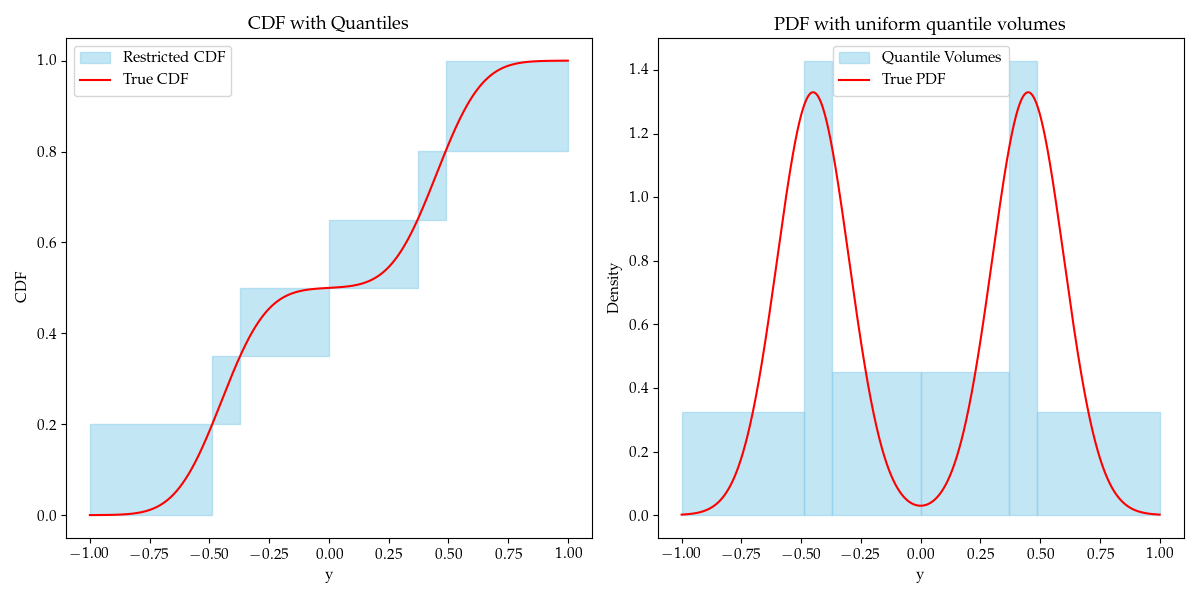
\includegraphics[width=0.8\textwidth]{resources/restricted_pdf_cdf_with_qr5.png}\label{fig:restricted_pdf_cdf_with_qr5}
    }\\
    \subfloat[Restricted CDF with 30 quantiles]{
        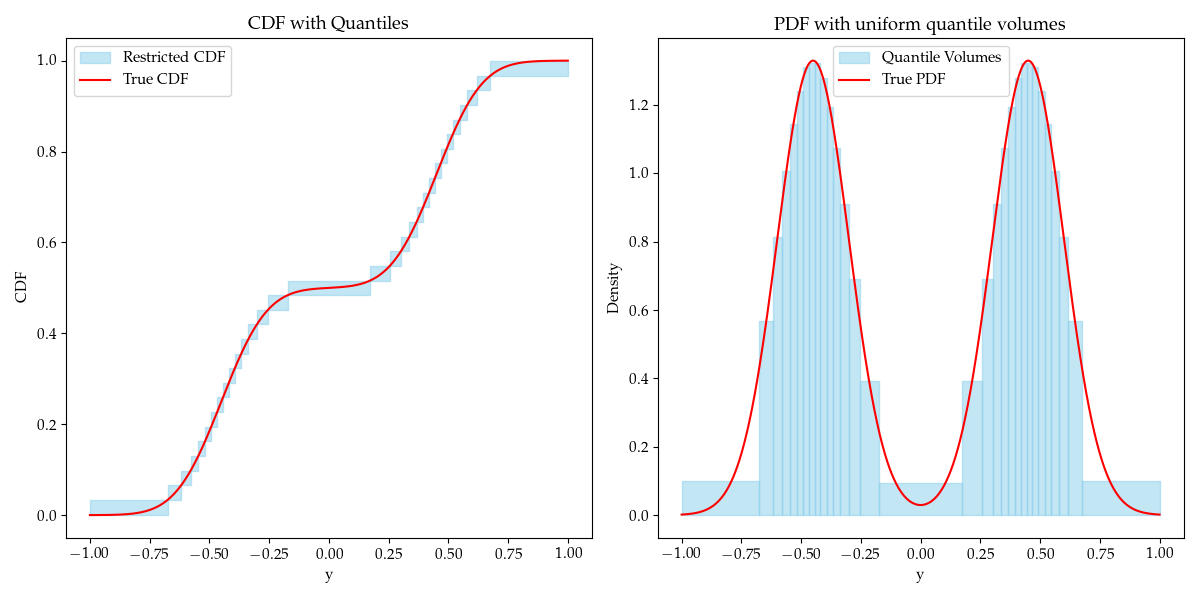
\includegraphics[width=0.8\textwidth]{resources/restricted_pdf_cdf_with_qr30.png}\label{fig:restricted_pdf_cdf_with_qr30}
    }

    \caption[Restriction on the CDF with multiple Quantile Regression]{Restriction on the CDF with multiple Quantile Regression. It is apparent that as we increase the number of quantiles that we predict, the restriction on the CDF becomes more and more stringent. Moreover, we approach the true PDF on the right side if using a smoothness assumption, in this case uniform.}
\end{figure}

We can now infer quite clearly what information is required in a $\mathscr{P}_{\theta}$ in order to do CP, QR or CDE.\@ For QR, it is sufficient to know that
$\forall \mathbf{x} \in \mathbb{R}^n \exists q \in (0,1) \forall p\in \mathscr{P}_{\theta}(\mathbf{x}): \int_{-\infty}^{Q(\mathbf{x})} p d\mathbf{y} = q$, as intuitively depicted in \fef{fig:restricted_pdf_cdf_with_qr5}. Although the full PDF is unknown when observing only the restricted PDF, we can still unambiguously determine specific quantile levels. For CP, if we want to be conditionally calibrated as described in \pef{sec:calibration_cp}, we need to know that $\forall \mathbf{x} \in \mathbb{R}^n \exists \alpha \in (0,1) \forall p\in \mathscr{P}_{\theta}(\mathbf{x}): \int_{C(\mathbf{x})} p(\mathbf{y}) d\mathbf{y} = 1 - \alpha$. In \fef{fig:restricted_pdf_cdf_with_qr5} we can see that this could simply be an interval between two quantile levels that we predict. If we only require marginal calibration we only need to know that this is true in expectation over $\mathbb{R}^n$ which is a weaker restriction. For CDE we need to know that $\forall \mathbf{x} \in \mathbb{R}^n: |\mathscr{P}_{\theta}(\mathbf{x})| = 1$. Because of this, also practically it is quite clear that there is no ambiguity in predicting quantiles or CP regions if we already have a CDE kind of restriction $\mathscr{P}_\theta$.

From this we can already see a way in which all CPM are the same task, that is they all aim to restrict the PDF $\mathcal{P}$. With that we already showed a very fundamental statement of this work. However, in order to be able to obtain $\mathscr{P}_\theta$ such that it is valid for CDE via CP or QR, and thus being able to infer each of CP, QR and CDE from the other, we need to be able to restrict it to be a single element with CP and QR.\@ Therefore, we need to observe that we can just apply multiple QR or CP restrictions to $\mathscr{P}_\theta$ by performing multiple CDM that only partially restrict $\mathcal{P}$ for each $\mathbf{x}\in\mathbb{R}^n$:

\begin{equation}
    \forall x\in\mathbb{R}^n: \mathscr{P}_{\theta}(x) = \bigcap_{i=1}^n \mathscr{P}_{\theta_i}
\end{equation}

Where each $\mathscr{P}_{\theta_i}$ is a restriction on $\mathcal{P}$ that is valid for CDE, CP or QR.\@ Thereby one needs to be careful in the definition of each restriction not to have two restrictions that contradict each other and thus produce the empty set, however this is generally approximately possible in practice because of the asymptotic properties of the CDMs. Moreover, even if we have two model producing functions that contradict each other, practically that often is not a problem. For example if we do multiple quantile regression and observe quantile inversion, then it is a common practice to simply swap the two quantiles out. In this case in is common practice to just take this then as the final $\mathcal{P}_{\theta}$.\footnote{This common practice, while it results in a valid $\mathcal{P}_{\theta}$ does generally and also in literature lack a theoretical foundation an is more a `trick of the trade'. We will not analyze the theoretical validity of doing this.} Moreover, combining restrictions of $\mathcal{P}_\theta$ implicitly is already a common method in the literature, e.g.~\cite{sesia2021conformal} where multiple quantile regression is used in order to obtain a grid of quantiles that can be used to infer CP regions.

We can arbitrarily restrict $\mathcal{P}_\theta$ if we can make those restrictions arbitrarily tight with a method as we can also see in \fef{fig:restricted_pdf_cdf_with_qr30}. In the case of QR we can simply make an infinitely dense quantile grid which accomplishes that. That is, in the limit of the number of quantiles torwards infinity the requirement for CDE will be fullfilled. It is easy to see, since in the limit for each quantile $q\in(0,1)$ we will have a unique quantile and from that we can clearly infer the PDF uniquely, that is, from the quantile function we can recover the PDF.\@

For CP it is a bit less obvious since we could define CP intervals anywhere and it is unclear how we would make sure that we still restrict everything even if we increase/decrease the confidence level. However, most if not all CP methods in the literature (e.g.~\cite{sesia2021conformal, chernozhukov2021distributional}) are based on methods that allow for a nested way of increasing/descreasing CP regions which relates to how calibration works in CP as we can see in \pef{sec:recalibration_cp}. Nested regions essentially allow that we indirectly also obtain all quantile levels precisely and thus also the PDF.\@

Notably, methods that derive CDE from QR or CP are only approximate and asymptotic in both the size of the dataset and the number of restrictions imposed. Similarly, CDE techniques themselves are asymptotic in the data and not fully expressive in practice. Particularly under \sref[Assumption]{def:model_producing}, it is implied that CDE cannot be completely accurate with finite data, thereby necessitating some flexibility in PDF restriction even within CDE methodologies. This uncertainty in the restriction that must necessarily be present due to limited data and \sref[Assumption]{def:model_producing} is effectively due to epistemic uncertainty which is treaded in more depth in \pef{sec:uncertainty_calibration}. This completes the argument that CDE, CP and QR are fundamentally the same task, that is, restricting the PDF $\mathcal{P}$ in a way that we can infer the desired target type from it and we can use techniques from one method for the other methods or more generally that implicitly we are always only restricting the PDF $\mathcal{P}$ and from that we can under certain conditions infer the desired target type.

Moreover, in practice if we want to obtain the CDE target from a not fully restricted $\mathcal{P}$ we can simply make smoothness assumptions, since we need to do that anyways as described in \pef{sec:smoothness} and implicitly also designated CDE methods do that as can be seen from the argment above that also CDE methods practically need some freedom in the restriction of the conditional PDF, which we will not go into more depth in this work.

The theoretical underpinnings of $\mathscr{P}_\theta$ are inherently self-evident, rendering a formal proof superfluous, in contrast to the assertions put forth in \pef{sec:connection_model_producing}. This intrinsic property stems from the very definition of the methods employed, implying that the mere presence of CP, QR, or CDE inherently imposes constraints on the universe of admissible probability density functions. Despite the profound implications of this observation, it has hitherto remained unexplored in the extant literature, to the best of our knowledge. The significance of this insight lies in the novel lens it provides for understanding and interpreting CP, QR, and CDE, potentially unveiling new avenues for theoretical and practical advancements in these domains.

\subsection{CDM to improve CP and QR*}
In this work we argue, that by first estimating a more holistic picture of the true conditional density via $\mathscr{P}_\theta$ instead of being ignorant to the implicit restrictions on the conditional PDFs we can improve the performance of CP and QR.\@ Specifically, a tighter restriction of $\mathcal{P}$ for each $\mathbf{x}\in\mathbb{R}^n$ has a regulatory effect that eliminates implausible partial predictions. Conceptually, this is akin to an ensemble method achieved through extensive quantile regression, CP or CDE.\@

For instance, predicting a quantile at an imprecise position can be stabilized by implementing a dense quantile regression grid spanning the entire interval $(0,1)$. This approach likely prevents quantile inversion, thus allowing for the adjustment (via swapping/sorting) of quantiles to derive a valid PDF, applicable analogously to CP.\@

Moreover, this approach empirically enhances the CP/QR models, as demonstrated in the experiments referenced in \pef{sec:experiment_results_more_restriction}. By incorporating additional segments of the PDF $\mathcal{P}_{\theta'}$—used as a regularizer—we observe no overall degradation in performance. For example, targeting solely the median does not compromise accuracy, even if the 0.1 and 0.9 quantiles are also predicted and utilized as regularization parameters. It is important to note, however, that while these additional predictions generally improve model robustness on average, they might lead to suboptimal outputs for specific samples. Nevertheless, the aggregate effect tends to be positive, reinforcing the utility of this comprehensive modeling approach.

\subsection{Reassessing the `Distribution-Free' Nature of CP Methods*}

In the literature, CP methods are often lauded for their distribution-free nature, implying no distributional assumptions are made within the model~\cite{angelopoulos2021gentle}. This characteristic is highlighted as a theoretical advantage since it suggests the ability to predict aspects of any arbitrary conditional PDF, ostensibly showing CP's superiority over methods like CDE e.g.\ via MDNs.

However, this notion of being distribution-free or not is nuanced. On the one hand, even if we introduce distributional assumptions in CDE methods like MDNs, in fact, it can be shown that when using MDNs for CDE with an infinite number of Gaussian components, we can predict any arbitrary PDF~\cite{bishop1994mixture}. On the other hand, so called distribution free CP methods, when limited to a finite number of model parameters—as it is always the case in practice—similarly have distributional assumptions introduced by the modeling limitations of NNs. For NNs those modeling limitations are present in the initialization of weights with a certain distribution and the distribution of activations after linearities and activation functions. This is evident when considering works by~\cite{klambauer2017self, ioffe2015batch} that analytically display the distributions inherent in NNs, however, this concept clearly extends to arbitrary methods beyond NNs. We can conclude that both, CP and CDE, are distribution free and not distribution free methods simply depending on the perspective if we allow infinite expressivity of the model or not respectively.

Moreover, the claim that being distribution-free offers practical advantages is debatable. Arguably, this merely implies infinite model expressivity, which contradicts the practical requirement for model smoothness as discussed in \pef{sec:smoothness}. In practice, no CP method truly avoids making distributional assumptions, rendering the supposed benefits of being distribution-free moot.

\subsection{Limitations of the Bridge between CDMs}

While the statements made about CDE, CP, and QR being analogous tasks are valid under the conditions specified in \sref[Assumption]{def:assumptions}, this may not always be the case. Absent these assumptions, it is reasonable to suspect that these statements generally hold in practice, albeit with some limitations. For instance, the conditional CDF may exhibit discontinuities, flat spots, or zero-density intervals, which could challenge all three methods. Specifically, QR may yield unpredictable results when encountering a jump in the CDF at the quantile level it aims to estimate. Nonetheless, we can approximate any conditional PDF that does not meet our assumptions with one that does, thus supporting the practical applicability of these statements.

Furthermore, methods like quantile swapping with quantile inversion, which are used to maintain a valid PDF while integrating constraints, are underexplored and impose somewhat arbitrary assumptions on the PDF.\@ However, given that all CDMs asymptotically converge to the true conditional CDFs, in the sense that the imposed restrictions will still be containing the true conditional CDFs, under the \sref[Assumption]{def:model_producing} we adopt, discrepancies due to these constraints are typically artifacts of limited data. In such cases, approximate solutions are employed, mitigating what might otherwise be viewed as a limitation. Nevertheless, establishing a more theoretical basis for these methods would be beneficial.

The final limitation concerns our earlier demonstration in \pef{sec:connection_model_producing}, which posits a plausible hypothesis on why the model-producing function should handle sub-tasks of CDE, CP, and QR.\@ Despite presenting clear evidence supporting this hypothesis, a rigorous mathematical proof is absent and is identified as an area for future research. Nonetheless, the existing evidence provides a strong basis for this claim.

\subsection{Conclusion on the Bridge between CDMs}

From \pef{sec:bridge_cde_qr}, \pef{sec:bridge_cde_qr} and \pef{sec:cde_sub_cp_qr} we can see that the implicit task of CDMs is restricting on the sets of all possible PDFs $\mathscr{P}_\theta$. This has two major implications:

Firstly, any technique on a CDM implicitly acts on the corresponding $\mathscr{P}_\theta$ and thus can be thru $\mathscr{P}_\theta$ translated to any other CDM.\@ Consider, for example, a function intended to slightly increase the standard deviation within a CDE model across all $\mathbf{x} \in \mathbb{R}^n$ using $h(p) = 2p$. This adjustment in the CDE model reflects directly on $\mathscr{P}_\theta$, allowing for a generalized form of $h$ that explicitly acts on $\mathscr{P}_\theta$ and is applicable across different CDMs. Specifically, for an $\mathbf{x} \in \mathbb{R}^n$, the transformation is defined as $h(\mathscr{P}_{\theta}(\mathbf{x})) = \left\{2 p: p \in \mathscr{P}\theta(\mathbf{x}) \right\}$, which effectively applies $h$ to each element in $\mathscr{P}_\theta(\mathbf{x})$. Thus, techniques applied within one CDM can be translated to any other CDM using this approach.

Secondly, objectives achievable within one CDM can be accomplished using any other CDM.\@ For instance, obtaining a full conditional PDF can be realized through methods that involve QR or CP within any CDM framework.

\section{Optimal Conformal Prediction}\label{sec:optimal_cp}

In this section we first define what we mean by optimal CP and then show how we can infer optimal CP from CDM by using a novel method in this context. We will give a new perspective on the optimization objective of CDMs, which often is likelihood, and show how it relates to the definition of optimal conformal prediction that we give here. This relationship is of theoretical interest and also has practical implications as we will show in \pef{sec:calibration}.

To articulate our definition of optimal CP, we draw on the work of~\cite{sesia2021conformal}, where optimal CP is characterized by its ability to predict the shortest intervals for a specified miscoverage level, $\alpha$. Rather than predicting single intervals, we propose it is both simpler and more practical to target the smallest possible regions in the target space that, in expectation, contain the target variable with the requisite confidence level.

Let $\alpha \in (0,1)$ be a significance level. Then the goal of conformal prediction is to find a function $C : \mathbb{R}^n \to \mathcal{B}(\mathbb{R}^m)$ that can predict the subsets with the smallest Lebesgue measure $\lambda$ marginalized over $\Omega$ with significance $\alpha$. That means, formulated as a constrainted optimization problem, we want:
\begin{align}
    \min_U \quad      & \int_{\mathbb{R}^{m + n}} p(\mathbf{z})
    \lambda(C(\mathbf{x}))
    d\mathbf{z}
    \\
    \text{s.t.} \quad & \int_{\mathbb{R}^{m + n}} \mathds{1}_{\mathbf{y} \in
    C(\mathbf{x})} d\mathbf{z} = a
\end{align}

In particular, in the context of this \pef{sec:optimal_cp} we always assume that we have infinite data as we aim to show an asymptotic result. In the following \pef{sec:optimal_cp_proofs} we will introduce a new way to infer conformal regions and show a new perspective on the optimization objective of CDMs in the form of \sref[Theorem]{thm:optimal_cp}.

\subsection{New perspective on MLL and Optimal CP*}\label{sec:optimal_cp_proofs}

The method to infer the intervals that will be used by us is by utilizing the Highest Density Regions (HDR). Using this we can, given a PDF, infer the set of intervals with the shortest summed Lebesgue measure. In particular, we are shifting our focus from looking at the shortest regions to looking at the regions that contain the most probability mass, even tho that is very similar and mostly the same with HDR there are some delicate differences. This is partiularly beneficial since regions with high densities should usually not be ignored in practice as they often indicate important events as we will discuss in depth in \pef{sec:density_focus}

If $C$ is being calculated by first using a CDM to sufficiently restrict $\mathscr{P}_\theta$ in the sense of \pef{sec:cde_sub_cp_qr} and then using HDRs as defined by~\cite{hyndman1996computing} to obtain a significance level of $\alpha$, then $C$ is a function of the CDM and the significance level $\alpha$. HDR is by~\cite{hyndman1996computing} defined as:

\[
    H\left(f_a\right)=\left\{\mathbf{y}: f(\mathbf{y}) \geq f_a\right\}
\]
with
\[
    f_a = \max_{f_a} \left\{f_a \in \mathbb{R^+}: \mathbb{P}\left(\mathbf{y}
    \in
    H(f_a)\right) \geq a \right\}
\]

but it can be written equivalently as below. The below formulation is also the one being used in this work from now on.

\begin{equation}
    H\left(f, a\right):=\left\{\mathbf{y} \in \mathbb{R}^m: f(\mathbf{y}) \geq
    \max_{b} \left\{b \in \mathbb{R^+}: \mathbb{P}\left(\left\{\mathbf{\hat{y}}
    \in
    \mathbb{R}^m: f(\mathbf{\hat{y}}) \geq b\right\}\right) \geq a
    \right\}\right\}
    \label{eq:HDR}
\end{equation}

where $f$ is an arbitrary probability density function (PDF) and $a := 1 - \alpha$ is the confidence level. Note that $\mathbb{P}$ here is different from the one defined in the beginning and only here for defining HDRs. As the CDM in my case is parametric like MDNs it is more reasonable to write $C$ a function of the parameterization of the CDM and the coverage level. So considering that, the initial goal of conformal prediction can be rewritten as:

\begin{align}
    \min_{\theta \in \Theta} \quad & \int_{\mathbb{R}^{m + n}} p(\mathbf{z})
    \lambda(H(p(\mathbf{\hat{y}} \mid \mathbf{x}; \theta), a))
    d\mathbf{z} \label{eq:optimal_cp_obj_func}
    \\
    \text{s.t.} \quad              & \int_{\mathbb{R}^{m + n}}
    \mathds{1}_{\mathbf{y} \in
    H(p(\mathbf{\hat{y}} \mid \mathbf{x}; \theta), a)} d\mathbf{z} = a
\end{align}

where it is important that the $\mathbf{\hat{y}}$ is not the one we integrate over but more a demonstrative artefact we write to denote that $p(\mathbf{\hat{y}} \mid \mathbf{x}; \theta)$ is a conditional density. Moreover $\Theta$ is the space of all parameters of the CDE method.

In the following if we write $p(\mathbf{\hat{y}} \mid \mathbf{x}; \theta)$ we mean the PDF that can be inferred from a restriction of a CDM method parameterized with $\theta$ (see \pef{sec:cde_sub_cp_qr} for more details) and if we write $p(\mathbf{\hat{y}} \mid \mathbf{x})$, the true conditional density is meant. Notice, that the goal of this optimization problem is to optimize w.r.t.\ $\theta$ as it is basically the component that completely defines $p(\mathbf{\hat{y}} \mid \mathbf{x}; \theta)$. This in turn means we need to find the argmin of the optimization in \eef{eq:optimal_cp_obj_func}.

Let $\theta^*$ be the argmin of the equation in \eef{eq:optimal_cp_obj_func}, we would like to show that

\begin{equation}
    \theta^* = \argmax_{\theta \in \Theta}  \int_{\mathbb{R}^{m + n}}
    p(\mathbf{z}) \log p(\mathbf{y} \mid \mathbf{x}; \theta) d
    \mathbf{z}
\end{equation}

which is the maximum likelihood estimator (MLE), i.e.\ the model with the highest likelihood. This is of great importance if we wish to optimize a CDE method w.r.t.\ the maximum likelihood objective function in order to implicitly optimize for the conformal prediction objective function when using HDRs. In order to show this powerful statement we first need to develop some insight into the workings of the components in conformal prediction.

First, we require to show that $\lambda(H(p, a))$ is continously differentiable a.e.\ in order to make sensible statements. Its not that the intuition does not hold if its not continous, however, it complicates things and makes the statemtent more difficult. First in \sref[Lemma]{lem:continuity} below we show that this is fullfilled if the PDF fullfills our standard assumptions in \sref[Assumption]{def:assumptions}.

\begin{lemma}\label{lem:continuity}
    Let \(p: \mathbb{R}^m \to \mathbb{R}\) be a probability density function for which \sref[Assumption]{def:assumptions} hold where we neglect the $\mathbf{x}$ for brevity, i.e.\ we look at the PDF for any fixed $\mathbf{x}$.

    Furthermore let $p$ be for the random variable $\mathbf{Y}$ (for brevity we neglect the index) and let $g(b) := \mathbb{P}(p(\mathbf{Y}) \geq b)$. Moreover, $\lambda_p:[0, 1] \to \mathbb{R}$ with $\lambda_p(a) = \lambda(H(p, a))$. Then the following statements hold for $a \in (0,1)$:

    \begin{enumerate}
        \item $g(b)$ is strictly monotonic on the set $g^{-1}((0,1))$.
        \item $g(b)$ is continous.
        \item $g(b)$ is bijective on the set $g^{-1}((0,1))$.
        \item $g(b)$ is continously differentiable a.e.
        \item $B(p, a)$ is strictly monotonous on the set $B^{-1}((0,1))$.
        \item $B(p, a)$ is continous.
        \item $B(p, a)$ is bijecitve on the set $B^{-1}((0,1))$.
        \item $B(p, a)$ is continously differentiable a.e.
        \item $\lambda_p(a)$ is strictly monotonous.
        \item $\lambda_p(a)$ is continous.
        \item $\lambda_p(a)$ is bijective on the set $\lambda_p^{-1}((0,\infty))$.
        \item $\lambda_p(a)$ is continously differentiable a.e.
    \end{enumerate}
\end{lemma}

It is in particular required to not have any plateaus as in in \sref[Assumption]{def:assumptions} the PDF because otherwise per definition of HDR we can sometimes not obtain the shortest possible intervals for a confidence level $a$ since we would not know which part of the flat-spot to include in the interval and which to leave out.

\begin{proof}

    We will show all 12 implications in the following where several of the later statements are analogously to the first ones in a step by step fashion:
    \begin{enumerate}
        \item\label{item:monotonicity} Monotonicity is evident as the set \(\{\mathbf{Y} \geq b\}\) decreases when \(b\) increases. For strict monotonicity within \(g^{-1}((0,1))\), it must hold that \(\forall b \in g^{-1}((0,1))\), \(\frac{\partial \mathbb{P}(p(\mathbf{Y}) \geq b)}{\partial b} > 0\).

        Consider \(b \in g^{-1}((0,1))\). For any \(b' > b\), there exists an \(\epsilon > 0\) such that \(\mathbb{P}(p(\mathbf{Y}) \geq b + \epsilon) = \epsilon + \mathbb{P}(p(\mathbf{Y}) \geq b')\), ensuring a positive change in \(g\) over any interval, directly derived from the definition of the derivative. For any \(b'' \in (b, b')\), the continuity of \(p\) ensures a dense neighborhood around \(b''\) within \(p(\mathbf{Y}) \in (b, b')\), and by the Lebesgue Density Theorem, this neighborhood has positive measure, confirming strict monotonicity.

        \item\label{item:continuity} To demonstrate the continuity of \(g\), observe that due to the boundedness and monotonicity of the \(\mathbb{P}\) measure:
        \begin{equation}
            \lim_{b \downarrow \tilde{b}} g(b) = \mathbb{P}(\mathbf{Y} > \tilde{b})
        \end{equation}
        and
        \begin{equation}
            \lim_{b \uparrow \tilde{b}} g(b) = \mathbb{P}(\mathbf{Y} \geq \tilde{b})
        \end{equation}
        imply the continuity of \(g\) at \(\tilde{b}\) as long as \(\mathbb{P}(\mathbf{Y} = \tilde{b}) = 0\), which is an assumption.

        \item\label{item:bijectivity} Bijectivity follows from strict monotonicity directly. To be exact why actually $g^{-1}((0,1))$ exists for every $a \in (0,1)$ we can use the monotonicty of $g$ and the intermediate value therem since we can clearly find a $b$ such that $g(b)$ is arbitrarily close to $0$ and to $1$ because of the PDF property of $p$ and the fact that continuity of $p$ implies boundedness of $p$.

        \item\label{item:differentiability} Differentiability almost everywhere for \(g\) is deduced from Lebesgue's Theorem on Monotonic Functions, as \(g\) is monotonic. Continuous differentiability almost everywhere follows from \(g\) being uniformly continuous, as established by the Heine-Cantor Theorem, implying the continuity of its derivative almost everywhere.

        \item\label{item:monotonicity2} This follows by observing that $g$ is bijective on $g^{-1}((0,1))$ which implies that the maximum of $b$ where $g$ is still greater-equal $a$ will always exactly reach $a$. Then since $g$ is $g^{-1}((0,1))$ is well defined and $g$ is strictly monotonic we see that increasing $a$ will always increase the possible $b$.

        \item\label{item:continuity2} Continuity follows from the fact that $g$ is also continous and bijective as we learned from~\sref[Step]{item:continuity} and~\sref[Step]{item:bijectivity}.

        \item Bijectivity follows directly from~\sref[Step]{item:monotonicity2} and~\sref[Step]{item:continuity2} similar to~\sref[Step]{item:bijectivity}.

        \item Follows with the same logic as~\sref[Step]{item:differentiability}.

              \item\label{item:monotonicity3} Strict monotonicity of $B$ and the same argument as in~\sref[Step]{item:monotonicity}. (Lebesgue density theorem) imply this.

        \item This can also be shown by the same argument as~\sref[Step]{item:continuity} and continuity of $B$ in~\sref[Step]{item:continuity2}.

        \item Bijectivity follows from~\sref[Step]{item:monotonicity3}. The fact that the image is $(0,\infty)$ follows from the fact that $p>0$ and thus in order to go with $a \to 1$ we will require infinite area in the Lebesgue sense. That we also approach $0$ in the image follows easily from bijectivity of $B$ on $(0,1)$.

        \item Follows analogous to~\sref[Step]{item:differentiability}.

    \end{enumerate}
\end{proof}

From \sref[Lemma]{lem:continuity} we can see that if the PDF is continously diffentiable a.e., also the length of the HDR w.r.t.\ $a$ will be continously differentiable a.e.. This is required because otherwise we can not show the following lemma about convexity of the HDR length w.r.t.\ $a$:

\begin{lemma}
    Let \(p: \mathbb{R}^m \to \mathbb{R}\) fullfill \sref[Assumption]{def:assumptions}. Then, the function $\lambda_{p}(a)$ is strictly convex, i.e.,

    \begin{equation}
        \frac{\partial^2 \lambda_{p}(a)}{\partial a^2} > 0.
    \end{equation}

\end{lemma}
\begin{proof}
    Without loss of generality, assume \(a_1 < a_2\) with both \(a_1, a_2 \in (0,1)\). For any \(\alpha \in (0, 1)\), let \(a := \alpha a_1 + (1-\alpha) a_2\). By the definition of \(H_p\) in \eef{eq:HDR}, the set \(H(p, a)\) encompasses points up to the highest densities corresponding to coverage \(a\). Taken from the definition in \eef{eq:HDR} we define this highest density as

    \begin{equation}
        B(p, a):=\max \left\{b \in \mathbb{R^+}: \mathbb{P}\left(\left\{\mathbf{\hat{y}}
        \in
        \mathbb{R}^m: p(\mathbf{\hat{y}}) \geq b\right\}\right) \geq a
        \right\}
    \end{equation}

    This implies that \(\lambda_{p}(a_1) \leq \lambda_{p}(a) \leq \lambda_{p}(a_2)\). Define $k_1 = a-a_1$, $k_2 = a_2 - a$. Consequently, \(H(p, a_1) \subset H(p, a)\), indicating that to transition from \(H(p, a_1)\) to \(H(p, a)\), only points with density less than $B(p, a_1)$ can be utilized. In contrast, if we go from $a$ to $a_2$ only points with a density less than $B(p, a)$ can be utilized.

    As we know that
    \begin{equation}
        \lambda_p(a) = \lambda(H(p, a_1) \cup (H(p,a)\setminus H(p,a_1))) = \lambda_p(a_1) + \lambda(H(p,a)\setminus H(p, a_1))
    \end{equation}
    and we know that $\lambda(H(p,a)\setminus H(p, a_1)) \leq k_1 \cdot B(p, a)$ and $\lambda(H(p,a_2)\setminus H(p, a)) \geq k_2 \cdot B(p, a)$ we can see that we can approximate the gradient by dividing the change of $\lambda_p$ by the change of $a$, which is in $k_1$ and $k_2$ we see that the gradients are bounded from above and below respectively for the invervals $(a_1, a)$ and $(a, a_2)$. Moreover strict monotonicity of $B$ as shown in \sref[Lemma]{lem:continuity} implies that the gradient is strictly increasing for $\lambda_p$ which implies a postive second derivative and thus convexity.

    In particular, the second derivative exists by the use of the Lebesgue's Theorem for Monotonic Function a.e.\ since the first derivative exists continuously a.e.\ and is strictly monotonic as we know from \sref[Lemma]{lem:continuity} which implies absolute continous derivative a.e.\ and thus twice differentiability a.e.. This completes the proof.
\end{proof}

\begin{lemma}\label{lem:hdr_optimality_mll}
    For any PDFs $f: \mathbb{R}^m \to \mathbb{R}$ and $p: \mathbb{R}^m \to \mathbb{R}$, where $p$ must fullfill \sref[Assumptions]{def:assumptions}, with the same coverage size under confidence levels $a_p$ and $a_f$, that is,

    \begin{equation}
        \lambda_f(a_f) = \lambda_p(a_p)
    \end{equation}

    it holds that if we measure the coverage of those HDRs with samples distributed w.r.t.\ $p$, that the coverage measured with $H(p,a)$ will be greater-equal. Moreover, the coverage level of $H(p,a)$ will be exactly $a_p$. Formally:

    \begin{equation}
        \int_{\mathbb{R}^{m}} p(\mathbf{y}) \mathds1_{\mathbf{y} \in H(f, a_f)} d
        \mathbf{y} \leq \int_{\mathbb{R}^{m}} p(\mathbf{y})
        \mathds1_{\mathbf{y} \in
            H(p, a_p)} d \mathbf{y} = a_p
    \end{equation}
\end{lemma}
Note that it is absolutely possible that $a_p = a_f$.
\begin{proof}
    We split $H(p,a_p)$ and $H(f, a_f)$ into subsets: $H(f, a_f) = A \cup B$ and $H(p, a_p) = A \cup C$ with $H(f, a_f) \cap H(p,a_p) = A$, $H(f, a_f)\setminus A = B$ and $H(p, a_p)\setminus A = C$.

    \begin{equation}
        \int_{\mathbb{R}^{m}} p(\mathbf{y}) \mathds1_{\mathbf{y} \in H(f, a_f)} d
        \mathbf{y} = \int_{H(f, a_f)} p(\mathbf{y}) d \mathbf{y} = \int_{A}
        p(\mathbf{y})
        d \mathbf{y} + \int_{B} p(\mathbf{y}) d \mathbf{y}
    \end{equation}

    \begin{equation}
        \int_{\mathbb{R}^{m}} p(\mathbf{y}) \mathds1_{\mathbf{y} \in H(p, a_p)} d
        \mathbf{y} = \int_{H(p, a_p)} p(\mathbf{y}) d \mathbf{y} = \int_{A}
        p(\mathbf{y})
        d \mathbf{y} + \int_{C} p(\mathbf{y}) d \mathbf{y}
    \end{equation}

    since the $A$ part of the integrals is equal we can ignore it for comparing $H(f, a_f)$ and $H(p, a_p)$ coverage. So, we need to show:

    \begin{equation}
        \int_{B} p(\mathbf{y}) d \mathbf{y} \leq \int_{C} p(\mathbf{y}) d
        \mathbf{y}
    \end{equation}

    This can be shown by proofing $\forall \mathbf{y}_B\in B \forall \mathbf{y}_C \in C: p(\mathbf{y}_B) \leq p(\mathbf{y}_C)$ because $\lambda(B) =  \lambda(C)$.
    So, let $\mathbf{y}_B$ and $\mathbf{y}_C$ be arbitrary from the corresponding sets. Then we know that $\mathbf{y}_B \in H(p,a_p)$, which means that $p(\mathbf{y}_C) \geq B(p, a_p)$ where $B(p, a_p)$ is the maximum density bound such that the coverage level of $a_p$ is still given w.r.t.\ $p$. However, since $\mathbf{y}_C \notin H(p,a_p)$ this means that $p(\mathbf{y}_C) < B(p, a_p)$, which shows the first part of the proof.

    The second part of the proof is to show that
    \begin{equation}
        \int_{\mathbb{R}^{m}} p(\mathbf{y}) \mathds1_{\mathbf{y} \in H(p, a_p)} d
        \mathbf{y} = a_p
    \end{equation}

    which follows from the fact that with our Assumption~\ref{def:assumptions} $B(p, a_p)$ is bijective and thus $\mathbb{P}(\mathbf{Y} \geq B(p, a_p)) = a_p$. In particular, $H(p, a_p)$ is per construction a set where this is fullfilled.
\end{proof}

In order to finally be able to use this lemma efficiently we need to define something like an inverse of the HDR w.r.t.\ the confidence level, which based on the input $\mathbf{x}$ and the length $\lambda(H(p(\mathbf{y} \mid \mathbf{y}), a))$ gives us the confidence level that we would need to insert in $H$ together with the true distribution at $x$ to obtain the same size of the distribution but with \sref[Lemma]{lem:hdr_optimality_mll} has a larger or equal coverage.

\begin{definition}[HDR Transform]\label{def:hdr_transform}
    Let $f,p : \mathbb{R}^m \to \mathbb{R}$ be two probability density functions and let $a \in (0,1)$ be some coverage level. Then we define the HDR Transform as:

    \begin{equation}
        H_p(f, a) := \max \left\{b \in (0,1):  \lambda_p(b) \leq \lambda_f(a)\right\}
    \end{equation}

\end{definition}
In words, the HDR Transform gives us the maximal significance level that we can insert under the distribution $p$ while maintaining a coverage size lower-equal than what we obtain by inserting the significance level $a$ under the distribution $f$.

In particular, if we evaluate the actual coverage of $H(f, a)$ with samples drawn from $p$, then the coverage will be always lower-equal $a$ which follows from \sref[Lemma]{lem:hdr_optimality_mll}. The HDR transform then gives us the confidence level that we need to insert into the HDR with the true distribution to obtain the same coverage size but are guranteed to have higher-equal coverage.

Using this definition together with \sref[Lemma]{lem:hdr_optimality_mll} establishes a very powerful tool to make proofs related to HDR.\@ The following lemma is a direct consequence of the definition of the HDR Transform and \sref[Lemma]{lem:hdr_optimality_mll} and is the last piece of the puzzle to show \sref[Theorem]{thm:optimal_cp}

\begin{lemma}\label{lem:hdr_optimality}
    With $f,p$ as in \sref[Definition]{def:hdr_transform} and \sref[Assumption]{def:assumptions} on $p$, it always holds that:

    \begin{equation}
        H_p(f, a) = \max \left\{b \in (0,1): \lambda_p(b) = \lambda_f(a)\right\}
    \end{equation}

    and that the right hand side exists.
\end{lemma}
\begin{proof}
    Bijectivity of $\lambda_p(a)$, under the assumptions, with \sref[Lemma]{lem:continuity} implies that exactly one $b$ exists such that $\lambda(H(p, b)) = \lambda(H(f, a))$ which finishes the proof.
\end{proof}

Now, we have all the necessary tools to prove an important statement. Henceforth, the expectation $\mathbb{E}$ is used with respect to the entire sample space $\mathbb{R}^{m+n}$ and with the random variables $\mathbf{Y}$ and $\mathbf{X}$, which have the joint PDF $p(\mathbf{y}, \mathbf{x})$. Furthermore, if $\mathbf{\hat{y}}$ is mentioned, it is not as an input to a function but as a demonstrative artifact indicating that the function maps to a conditional density defined in the same space as $\mathbf{Y}$.

\begin{theorem}[MLL is equivalent with Optimal Conformal Prediction]\label{thm:optimal_cp}
    We want to show that if we have definitions as in \pef{sec:cp}, the space of all parameters $\Theta$ and $\forall \mathbf{x}\in\mathbb{R}^n: p(\mathbf{y}\mid \mathbf{x})$ fullfills \sref[Assumption]{def:assumptions} and that

    \begin{equation}
        \forall \mathbf{x}\in \mathbb{R}^n: \max_{\theta \in \Theta} p(\mathbf{y} \mid \mathbf{x}; \theta) = p(\mathbf{y} \mid \mathbf{x})
        \label{eq:assn_mle_is_true}
    \end{equation}

    then it holds that:

    \begin{equation}
        \argmax_{\theta \in \Theta}  \mathbb{E} \left[ \log
            p(\mathbf{Y} \mid \mathbf{X}; \theta) \right]
        \label{eq:maximum_log_likelihood}
    \end{equation}

    equals

    \begin{align}
         & \argmin_{\theta \in \Theta} \mathbb{E} \left[
            \lambda_{p(\mathbf{\hat{y}}\mid\mathbf{X}; \theta)}( a)
        \right]                                          \\
         & \text{s.t.} \quad \mathbb{E} \left[
        \mathds{1}_{\mathbf{Y} \in
        H(p(\mathbf{\hat{y}} \mid \mathbf{X}; \theta), a)} \right]
        = a
    \end{align}

\end{theorem}

Importantly, under our assumption in \eef{eq:assn_mle_is_true} we have that \eef{eq:maximum_log_likelihood} is the true underlying conditional distribution as a property of the MLE, i.e.\ $\forall \mathbf{x}\in\mathbb{R}^n: p(\mathbf{\hat{y}}\mid\mathbf{x}; \theta^*) = p(\mathbf{\hat{y}}\mid\mathbf{x})$. So \sref[Theorem]{thm:optimal_cp} not only shows an equality between the MLE and optimal CP but also an equality between the true underlying distribution and the underlying model of optimal CP.\@

\begin{proof}
    Let $\theta \neq \theta^*$ be arbitrary but fixed. If we can show that for this $\theta$ it holds that if

    \begin{equation}
        \mathbb{E} \left[ \lambda_{p(\mathbf{\hat{y}}\mid\mathbf{X};\theta)}(a)\right]
        <
        \left[\lambda_{p(\mathbf{\hat{y}}\mid\mathbf{X})}(a) \right]
        \label{eq:inequality_00}
    \end{equation}
    it implies
    \begin{equation}
        \mathbb{E} \left[ \mathds{1}_{\mathbf{Y} \in
        H(p(\mathbf{\hat{y}}\mid \mathbf{X}; \theta), a)} \right] < a
        \label{eq:inequality_01}
    \end{equation}

    then it would finish the proof, since it'd show that for any parameter set $\theta$, that produces a smaller average HDR than the the MLE, the constraint would be violated and it is clear that if using the MLE, which is the same as the true PDF, we would fulfill the constraint because of \sref[Lemma]{lem:hdr_optimality_mll}. We will show now that \eef{eq:inequality_00} $\implies$ \eef{eq:inequality_01}. So  $\theta$ is such that \eef{eq:inequality_00} holds.

    First, we can upper bound the coverage with the HDR transform in \sref[Definition]{def:hdr_transform}:

    \begin{equation}
        \mathbb{E} \left[ \mathds{1}_{\mathbf{Y} \in
        H(p(\mathbf{\hat{y}}\mid \mathbf{X}; \theta), a)} \right]
        \leq
        \mathbb{E} \left[ \mathds{1}_{\mathbf{Y} \in
        H(p(\mathbf{\hat{y}} \mid \mathbf{X}), H_{p(\hat{\mathbf{y}}\mid \mathbf{X})}(p(\mathbf{\hat{y}}\mid
        \mathbf{X};
        \theta), a))} \right]
        \label{eq:upper_bound}
    \end{equation}

    \begin{equation}
        = \mathbb{E}\left[H_{p(\hat{\mathbf{y}}\mid \mathbf{X})}(p(\mathbf{\hat{y}}\mid \mathbf{X}; \theta),
            a)
            \right]
        \label{eq:upper_bound_2}
    \end{equation}

    The upper bound follows directly from \sref[Lemma]{lem:hdr_optimality_mll} and the monotonicity property of integrals. The equality in \eef{eq:upper_bound_2} follows from the fact that if we evaluate the coverage w.r.t.\ underlying distribution $p$ we will always get the same coverage level as the one we inserted in the HDR if we fullfill \sref[Assumption]{def:assumptions}\footnote{This holds because the true PDF is always calibrated.}.

    We know that:
    \begin{equation}
        \mathbb{E}\left[\lambda_{p(\mathbf{\hat{y}}\mid\mathbf{X})}(a)\right] > \mathbb{E}\left[ \lambda_{p(\mathbf{\hat{y}}\mid\mathbf{X};\theta)}( a) \right]
        \label{eq:inequality_0}
    \end{equation}
    and
    \begin{equation}
        \mathbb{E}\left[ \lambda_{p(\mathbf{\hat{y}}\mid\mathbf{X}; \theta)}( a) \right]
        =\mathbb{E}\left[ \lambda_{p(\mathbf{\hat{y}}\mid\mathbf{X})}\left(
            H_{p(\hat{\mathbf{y}}\mid \mathbf{X})}(p(\mathbf{\hat{y}}\mid \mathbf{X}; \theta), a)\right)
            \right]
        \label{eq:inequality_1}
    \end{equation}

    where the second equality follows from \sref[Lemma]{lem:hdr_optimality}. This upper bound gives via \sref[Lemma]{lem:hdr_optimality} the highest coverage level for the same coverage size that is possible. If we can show the desired result for this upper bound, then we have shown the desired result.

    Due to convexity and with the Jensen inequality we now have that then we can appended to the equation in \eef{eq:inequality_1} the following inequality on the right:
    \begin{equation}
        \geq \mathbb{E}\left[ \lambda_{p(\mathbf{\hat{y}}\mid\mathbf{X})}\left(
            \mathbb{E}\left[H_{p(\hat{\mathbf{y}}\mid \mathbf{X})}(p(\mathbf{\hat{y}}\mid \mathbf{X};
                \theta), a)
                \right] \right)\right]
    \end{equation}

    and thus:

    \begin{equation}
        \mathbb{E}\left[\lambda_{p(\mathbf{\hat{y}}\mid\mathbf{X})}(a)\right]
        > \mathbb{E}\left[ \lambda_{p(\mathbf{\hat{y}}\mid\mathbf{X})}\left(
            \mathbb{E}\left[H_{p(\hat{\mathbf{y}}\mid \mathbf{X})}(p(\mathbf{\hat{y}}\mid \mathbf{X};
                \theta), a)
                \right] \right)\right]
    \end{equation}

    In words, what this means is that given the same distribution $p(\mathbf{\hat{y}}\mid\mathbf{x})$, we obtain a strictly larger average coverage size when using coverage $a$, then when we use coverage $\mathbb{E}\left[H_{p(\hat{\mathbf{y}}\mid \mathbf{X})}(p(\mathbf{\hat{y}}\mid \mathbf{x};\theta), a)\right]$. By monotonicity of the coverage size function, this means a.e.\ that

    \begin{equation}
        \lambda_{p(\mathbf{\hat{y}}\mid\mathbf{X})}(a) > \lambda_{p(\mathbf{\hat{y}}\mid\mathbf{X})}\left(
        \mathbb{E}\left[H_{p(\hat{\mathbf{y}}\mid \mathbf{X})}(p(\mathbf{\hat{y}}\mid \mathbf{X};
                \theta), a)
                \right] \right)
    \end{equation}

    since it can a.e.\ not be that the inequality is reversed and because of strict monotonicity of $\lambda_{p(\mathbf{\hat{y}}\mid\mathbf{X})}(a)$ which holds because of \sref[Lemma]{lem:continuity}. And thus we find that:

    \begin{equation}
        a > \mathbb{E}\left[H_{p(\hat{\mathbf{y}}\mid \mathbf{X})}(p(\mathbf{\hat{y}}\mid \mathbf{X};\theta), a)\right]
    \end{equation}

    where the right hand side, as we can see in \eef{eq:upper_bound}, upper bounds the coverage of the actual $p(\mathbf{\hat{y}}\mid \mathbf{X};\theta)$. This completes the proof.

\end{proof}
This result demonstrates our primary objective of \pef{sec:optimal_cp}: maximizing the likelihood in a CDE model and subsequently applying HDR to achieve small, yet calibrated regions, is equivalent to directly minimizing the HDR's size while ensuring calibration. Assuming that our CDE models can accurately approximate the true underlying distribution, this equivalence is a powerful outcome that allows us to concentrate solely on optimizing the likelihood for CDE while automatically yielding optimal conformal prediction with HDR.\@ This approach is notably more sophisticated than standard CP as described in \sref{sec:cp}, given it imposes a more complex requirement on the model, specifically, achieving the shortest possible HDR for a specified coverage level.

Furthermore, this analysis indicates that the MLE can be framed as a constrained optimization problem, echoing insights from~\cite{chung2021beyond}. Notably, this relationship is reciprocal; not only is the MLE the ideal model for optimal CP, but the optimal CP model also constitutes the optimal MLE model. This reciprocity directly stems from the equality established in \sref[Theorem]{thm:optimal_cp}. While this paper presents the concept as a theoretical insight, it may pave the way for significant empirical applications in future research. This interconnection possesses inherent mathematical elegance, illustrating that MLE naturally seeks the tightest possible peaks while maintaining calibration.

\subsection{Focusing on Density instead of the Coverage Level*}\label{sec:density_focus}

As suggested in \pef{sec:motivation}, this study proposes shifting the emphasis from merely the interval's length to the probability mass/density while lower bounding on the desired coverage level. The difference is subtle, but via \fef{fig:hdr_vs_shortest_intervals} we aim to provide a clear understanding of the difference through two distinct arguments:

Firstly, when performing CP, the focus is solely on minimizing the length of the single interval in the prediction while maintaining calibration, without considering the actual shape of the distribution. In particular, if it were possible to obtain significantly more probability mass with just a very slight increase the interval size it would be ignored. In the figure this can be observed when comparing the connected HDR with the shortest interval CP.\@ This scenario is illustrated in the figure, where using HDR followed by connecting disjoint intervals—as argued by~\cite{sesia2021conformal} to avoid multiple interval confusion—captures an additional peak that would otherwise be missed in a standard shortest interval CP approach. This example demonstrates that focusing exclusively on the length of the interval can lead to practically suboptimal results.

Secondly, the inclusion of a second peak in the CP prediction is advocated, even in the absence of empirical proof, because its identification by the model often indicates a substantial, distinct modality rather than a modeling artifact such as a heavy tail. Further research is necessary to substantiate this hypothesis.

Primarily for the first reason, and to a lesser extent the second, we argue that our approach (first applying HDR, then connecting the regions) offers advantages in practical scenarios such as healthcare and finance.

\begin{figure}
    \centering
    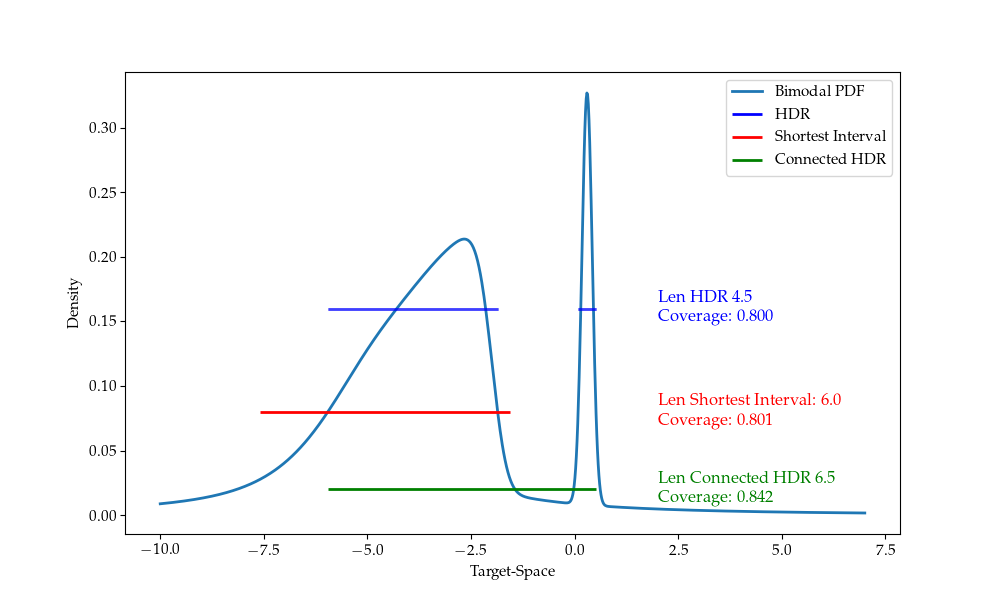
\includegraphics[width=0.8\textwidth]{resources/bimodal_distribution_hdr_vs_shortest_interval.png}
    \caption[Comparison of HDR, connected HDR and Shortest Interval CP]{Comparison of HDR, connected HDR and Shortest Interval CP for a bimodal distribution. We can see that although the connected HDR slightly overcoveres, we obtain significantly more coverage with only a slightly larger interval and also intutively this interval is more meaningful.}\label{fig:hdr_vs_shortest_intervals}
\end{figure}

\section{Calibration and Recalibration}\label{sec:calibration}

Calibration, while a core property of CP as described in \pef{sec:cp}, can in a more general way also be a desireable property of CDMs. In particular, we are calibrated in the context of $\mathscr{P}_\theta$ if for any quantile $q\in(0,1)$ that we choose, in expectation the proportion of the target that falls into the quantile really is $q$. CDMs often suffer from poor calibration in practice due to limited data, model misspecification, overfitting, or underfitting. For this section of our work we assume a limited training set $\mathcal{Z} = (\mathcal{X}, \mathcal{Y})$ that is used to train the CDM model. The probably most important realization on this is, that even tho the objective functions CDMs use in practice are optimal in theory, in practice we mostly need to resort to gradient based optimization methods, which require a step wise optimization and will only find local optima. Especially this insight is important because that means, even tho globally optimal models w.r.t.\ objective functions of CDMs will be calibrated, those objective functions do not guarantee calibration at all times during optimization. The reason is that the constraint of those optimization problems is an implicit one in practice and we will violate it usually with CP.\@

This is the reason why in practice recalibration methods exist and are at this time mostly applied to CP methods. From \pef{sec:cp_sub_cde} it follows that we can apply the same methods to all CDMs that are used currently only for CP.\@ However, since recalibration methods are mostly explored in CP methods, we will first introduce them in the context of CP in \pef{sec:calibration_cp} and step-wise extend the methods till we reach full generalization of recalibration in all CDMs in \pef{sec:calibration_cde_general}.

\subsection{Recalibration in CP}\label{sec:recalibration_cp}
Generally, calibration of CP refers to the requirement of the defining property of CP to be fullfilled as described in \pef{sec:calibration_cp}. In particular, since today most CP methods don't aim to estimate any CP intervals but specific ones, during optimization the calibration requirement is often overshadowed. However, calibration in the context of CP is basically the whole point of CP to begin with and because it is in practice often not fullfilled, recalibration methods are employed.

In any case, if doing recalibration we have that the estimated conformal intervals do in expectation not capture the desired $1 - \alpha$ proportion of the target in the calibration set. However, this can be tackled by recalibration for which a large possible number of methods exist, each depending on the method used to estimate the CP intervals.

To formally define calibration within CPs, consider the calibration objective function given by:

\begin{equation}
    \min_{\psi \in \Psi} |(1 - \alpha) - \mathbb{P}(\mathbf{Y} \in C(\mathscr{P}_{\theta}(\mathbf{X}), \psi))|
    \label{eq:calibration_objective_formal}
\end{equation}
This function aims to minimize the discrepancy between the desired confidence level \(1 - \alpha\) and the proportion of data within the CP interval predicted by the model, reflecting the model's calibration accuracy. Here $C$ is the map to the CP regions. $\psi\in\Psi$ is a configuration of the method used that can be optimized w.r.t.\ objective function and can be quite arbitrary and might dependent on the form of $\mathscr{P}_{\theta}$ which we argue for in \pef{sec:implicit_assumptions_cde}. In particular, $\psi$ is something that we apply after the CDM model has been estimated. We usually assume that we already have learned a CDM model estimated with parameters $\theta$ but that it is possibly not calibrated.

In the following we will describe a variation of $C$ and $\theta$ where we simplify the optimization problem in \eef{eq:calibration_objective_formal} to one that we can practically easily optimize, that is, it is a method that induces a misconformity score of sorts. The method we focus on here is heavily inspired by~\cite{sesia2021conformal} and can be used if $C$ and $\theta$ fullfill certain sufficient conditions:

\begin{definition}[Recalibration Requirements]\label{def:recalibration_requirements}

    Recalibration requirements with which we can easily optimize \eef{eq:calibration_objective_formal} are:
    \begin{enumerate}
        \item $C(\cdot,\psi)$ must be such that $\left(C\left(\cdot, \psi_r\right)\right)_{r \in \mathbf{R} \subsetneq \mathbb{R}}$ where $\mathbf{R}$ is bounded and $(C(\cdot,\psi_r))$ are strictly nested sets on the target space where the smallest set $(C(,\psi_0)) = \emptyset$ is the empty set and the largest one contains the full target space, i.e.\ we have $\forall r_1, r_2 \in \mathbf{R}: r_1 < r_2 \implies C(\cdot,\psi_{r_1}) \subset C(\cdot, \psi_{r_2})$.
        \item We require that the sequence is continous in a way if we want to be able to gurantee that we can come arbitrarily close to any desired calibration in expectation, i.e.\ $\forall a\in(0,1) \exists \psi\in\Psi : a = \mathbb{P}(\mathbf{Y} \in C(\mathscr{P}_{\theta}(\mathbf{X}), \psi))$
    \end{enumerate}
\end{definition}

Let $r$ be from the context of \sref[Definition]{def:recalibration_requirements}. Then, in words, requirement one means that we can, by tweaking $r$, obtain at least the empty set or the full target space and thus $0$ or $1$ coverage respectively. Requirement two means that we can interpolate $r$ such that we can reach any desired calibration in expectation. For example, the HDR with $a = r \in (0,1)$ fullfills this requirements under our standard assumptions \sref[Assumption]{def:assumptions} as explain in more detail in \pef{sec:cp_sub_cde_hrd}.

If condition two in \sref[Definition]{def:recalibration_requirements} is not fullfilled we can only gurantee that the calibration in expectation will be larger-equal the desired proportion. This is because there is guranteed to an $a$ close to $1$ that we can reach with an $r \in \mathbf{R}$ because of assumption one, so we might need to do with a converage larger than the desired one. When condition one is not fullfilled, we can not gurantee anything about the calibration in expectation, not even that it will be larger-equal the desired proportion. This is because there might be sets that are never part of the sequence but contain probability mass and thus we can never gurantee that we come even close to the desired calibration in expectation there.

If we optimize \eef{eq:calibration_objective_formal} on the calibration set, which is easily doable in practice with various methods since its just a convex univariate optimization problem with bounded domain, we can gurantee that the model is calibrated in expectation on the calibration set.

The $r$ required for a specific calibration sample in this \sref[Defintion]{def:recalibration_requirements} is basically a form of misconformity score. Thus the method used by~\cite{sesia2021conformal, chernozhukov2021distributional} and others is to basically sort the $r$ that are required for each single one of the calibration samples to be included in the CP interval. Then we take the upper $(1- \alpha)$ quantile of this sorted list as the $r$ that we use for the CP interval. We refer to~\cite{sesia2021conformal} for a more detailed explanation of the method and of it's validity, but it gurantees in expectation of both, the training and the validation set, that the CP interval will contain the desired proportion of the target. In particular, in this case $r$ acts as the conformity score of the sample as usually defined in CP literature like in the work by~\cite{sesia2021conformal}.

It is noteworthy, that if we have only few calibration samples, then the method will not work well, since the quantile will be very noisy. In this case the common choice is to resort to an overestimation, which means we take $r$ larger than the $1-\alpha$ quantile would suggest.

\subsection{Recalibration of CDE on CP when using HDR}\label{sec:cp_sub_cde_hrd}

As the HDR for a given confidence level $a$ is actually a sequence of nested sets which conform with assumptions from \sref[Definition]{def:recalibration_requirements} with $a = r \in (0,1)$ if we also have \sref[Assumption]{def:assumptions} applicable, for which it holds that those subintervals will contain $a$ proportion of the probability mass on the estimated conditional PDF, which can also be seen from \sref[Lemma]{lem:continuity}, which implies that we basically have a set of quantile intervals that sum up to $a$, we can see that a calibrated model will actually contain the true value in the HDR with a probability of $a$. Thus, if we are not calibrated, we can directly utilize the concepts described in \pef{sec:calibration_cp} when using HDR.\@

\subsection{Common Implicit Assumptions on the CP-Region Fuction*}\label{sec:implicit_assumptions_cp}

It is common practice in the CP literature to do calibration without of considering the implict assumptions that are being actually made when doing so. In particular the assumptions imposed on the $\mathscr{P}_\theta$ that we do CP with. One example would be that often in the literature we predict the 5\% and 95\% quantiles, and if we have a miscalibration we simply recalibrate the model by moving those two quantiles by the same amount in or outwards. Many assumptions are made there, in particular we assume that the conditional PDF is symmetric and that the densities of all samples look similar which are extremely strong assumptions also in practice. Furthermore, those assumptions might be orthorgonal to the optimization objective of CDM, i.e.\ to precisely model the true PDF asymptotically. We will now establish below in \pef{sec:shape_importance} a framework that allows us to do recalibration with theoretically justified assumptions.

\subsubsection{Likelihood and the Relation to CDMs}\label{sec:shape_importance}

It is clear that for CDE methods the likelihood is a very relevant metric and very often also the objective function in the optimization problem, e.g.\ for MDNs or KMNs. Moreover, from \pef{sec:cp_sub_cde} we can directly see that the likelihood must thus also be relvant for CDMs in general. Importantly, likelihood only directly can be evaluated on a specific PDF, but from \pef{sec:cde_sub_cp_qr} we inferred that CDM in general need to make smoothness assumptions anyways with arumentation from \pef{sec:smoothness} which at least makes directly sense if the CMDs are very restrictive on $\mathscr{P}_\theta$. However, the question arises how we can conceptualize likelihood if CDMs are not restricting $\mathscr{P}_\theta$ very much. In particular, can we make a statement that in any case a more accurate CDM method will allow for higher likelihoods in terms of the restrictive set of $\mathscr{P}_\theta$?

The optimization objectives of CDMs all have asymptotic gurantees on the restrictions they impose. Moreover, it is obvious that the likelihood and all other CDM metrics are optimal if the CMDs are restricted on the true conditional PDF as a property implicit in those metrics. However, it is not clear how exactly likelihood corresponds to other metrics used for restricting CDMs, like the pinball loss and it goes beyond the scope of this work to investigate which metrics are not only optmial at the same parameters but which are truly equivalent in terms of restrictions. For example, will a restriction that is better for the one metric always be better for the other metric?

In any case, we will leave it as a hypothesis that we generally have that good CDMs will have high likelihood which means in the scope of this work we designate likelihood as the general metric for CDMs. A good liklihood has certain desireable implications as properties of likelihood. In particular, we have the gurantee that in expectation on the entire target space the density will be close to the true density and if we have a model that generalizes, which we assume, then we also have that gurantee on unseen data.%make the assumption somewhere above more explicit

%TODO: I need to somewhere fit that this now implies that 1.better calibration => better likelihood 
\subsection{Calibration of CDMs in General*}\label{sec:calibration_cde_general}

We have in \pef{sec:calibration_cp} seen that it is possible in practice to recalibrate CP models. Now \pef{sec:cp_sub_cde} directly implies that we can generalize this concept to all CDMs, i.e.\ also to CDE and QR which is a core contribution of this work. Thereby we will with \pef{sec:shape_importance} also underpin the justification for common recalibration methods used in the literature~\cite{sesia2021conformal}.

In order to rigoriously utilize the theoretical framework that we have established, we first need to reformulate calibration for CP to a more general form that can be applied to all CDMs. Therefore we need to develop what recalibration means in the context of $\mathscr{P}_{\theta}$, i.e.\ the constrainted set of PDFs that any CP method is acting on.\\
As a sidenote, we want to make the connection to the foundational work of~\cite{gneiting2007probabilistic}, in particular to the concept of probabilistic calibration which when applicable to CMDs also implies that it is calibrated in the CP context in \pef{sec:calibration_cp}.

When we recalibrate, we essentially always admit that the current model $\mathscr{P}_{\theta}$ does not describe the true PDF accurately and in order to obtain a certain property, calibration that is, we effectively intend to change $\mathscr{P}_{\theta}$. In other words, we need to formulate what $C(\cdot, \psi)$ does in \eef{eq:calibration_objective_formal} as part of $\theta$, which defines the model, itself. This means we apply a function to the constrained sets of PDFs $\mathscr{P}_{\theta}$ to obtain a new set of PDFs $\mathscr{P}_{\theta'}$ that is calibrated or more generally that we apply the optimization problem in \eef{eq:calibration_objective_formal} to. By optimizing this we are essentially transforming this $\mathscr{P}_{\theta}$ w.r.t.\ $C(\cdot, \psi)$ such that a certain nested set gets assigned a different probability mass as before, in expectation, in the sense of \sref[Definition]{def:recalibration_requirements}. In a more general context of CDM, we have that when recalibrating we are moving quantiles within $\mathscr{P}_\theta$. As the quantiles directly encode all information required for producing the target types for the CDM that is the generalized interpretation of CP recalibration. %TODO: make figure for that!

\subsubsection{Practical Considerations for Recalibration of CDMs}

Practically to use this for e.g.\ CDE, one would simply define a dense grid of quantiles and then shift them all at once to recalibrate the model which will squeeze and stretch the model in the right places to obtain calibration. However, in order to realize a reasonable calibration with an infinitely dense grid of quantiles, we need to have an infinitely large calibration set. Interestingly, this limitation is not new to the general version of recalibration but actually also applies to CP which is easy to see. In practice we thus need to approximate recalibration. Moreover, it is noteworthy that, since recalibration acts on the quantiles and thus on the conditional CDF and not directly the PDF, we basically loose some amount of the smoothness of the estimated PDF when using designated CDE methods since we basically need to convert the PDF to a CDF by numerical integration and then after recalibration reconstruct the PDF from the CDF.\@ However, we have observed with a large enough grid size for inegration of the CDF that this is not a big problem in practice. Moreover, a practical considerations that could be made is that there are more samples at denser areas so we could use a denser grid there and a less dense grid in less dense areas for recalibration. Quantiles induced by the HDR as the quantile limits for recalibration fit this description well and this is also why we used the HDR for recalibrating empirically. Furthermore, the strongest limitation lies in the number of samples if the calibration set. In particular, if we only have few calibration samples it we can of course not precisely find the calibrated quantiles on a dense grid. Empirically we saw that it is helpful to do a smoothing operation with a filter size depending on the number of calibration samples but also depending on the problem after we recalibrate whole CDE models which can be justified with \pef{sec:smoothness}. A visualization of this can be seen in \fef{fig:recalibration_grid}. The smoothing operation that we employed was a moving average filter. Empirically it is very important to find the right windows size for the problem at hand, but the way to find this is not clear and might be a topic for future research. We only found that there is a dependence on the number of calibration samples.

\begin{figure}[htp]
    \centering
    \subfloat[Window Size = 1]{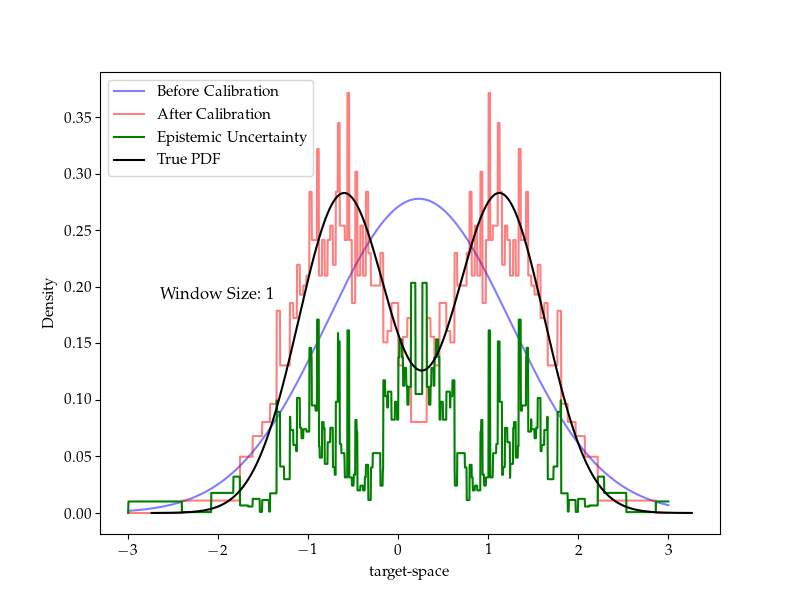
\includegraphics[width=0.5\textwidth]{resources/window_size_1.png}\label{fig:sub1}}
    \hfill
    \subfloat[Window Size = 51]{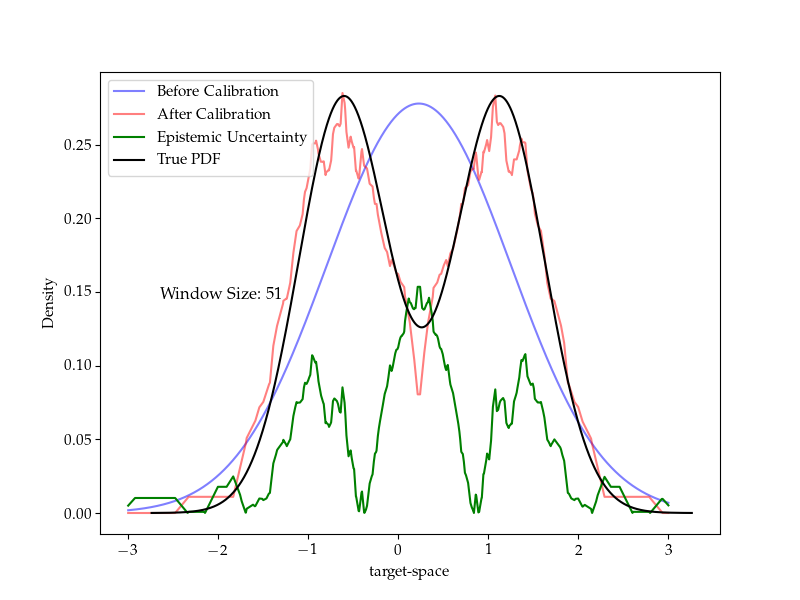
\includegraphics[width=0.5\textwidth]{resources/window_size_51.png}\label{fig:sub2}}
    \\
    \subfloat[Window Size = 101]{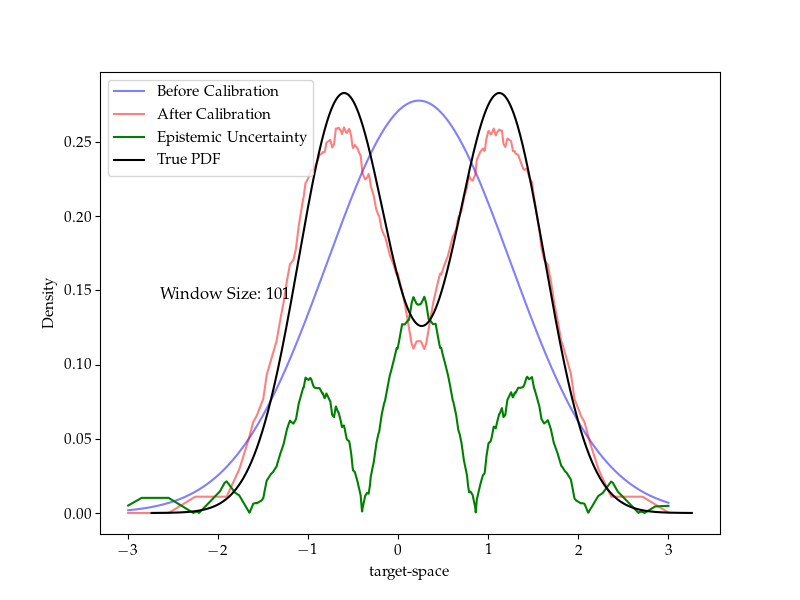
\includegraphics[width=0.5\textwidth]{resources/window_size_101.png}\label{fig:sub3}}
    \hfill
    \subfloat[Window Size = 401]{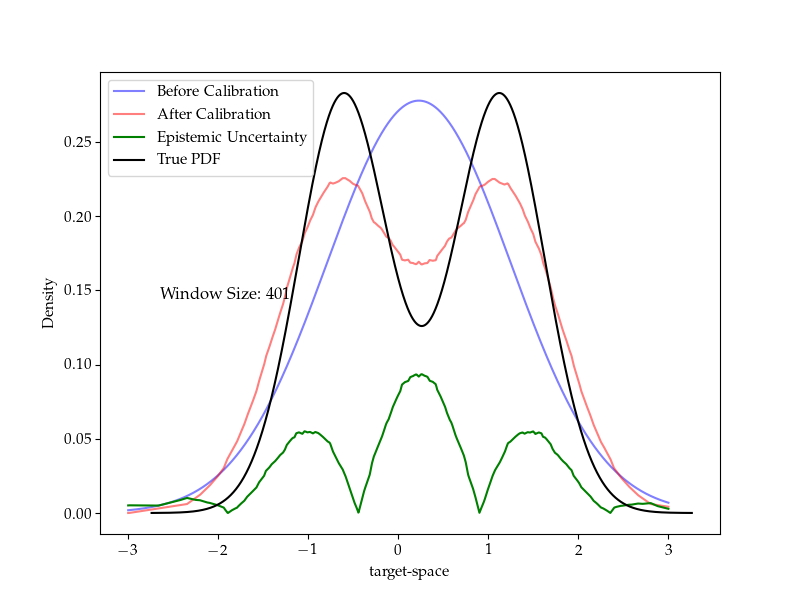
\includegraphics[width=0.5\textwidth]{resources/window_size_401.png}\label{fig:sub4}}
    \caption[Recalibration of a bimodal CDE model]{Recalibration of a bimodal CDE model. The model is recalibrated by shifting the quantiles of the HDR according to marginal misconformity quantile levels as in \sref[Algorithm]{alg:calibrate_pdf}. Moreover, we apply smoothing by using a moving average filter with different window sizes.}\label{fig:recalibration_grid}
\end{figure}

A Pseudo Code where we use HDR to recalibrate a CDE model is supplied in \sref[Algorithm]{alg:calibrate_pdf}.

\subsubsection{Implicit Assumptions when Recalibrating CDMs}\label{sec:implicit_assumptions_cde}

An important consideration for \pef{sec:calibration} is, that if we are changing $\theta$ arbitrarely in order to fullfill the optimization problem then, without considering the setting in a more general context, the only gurantee that we have is that the new $\mathscr{P}_{\theta'}$ is calibrated but might other than that not contain any relation to the true conditional PDF.\@ Further, this without a more general context this would be not more meaningful than trivial CP as described in \pef{sec:trivial_cp}.

However, with \pef{sec:shape_importance} we find that we must be close everywhere in the target space in expectation. With this methods like proposed by~\cite{sesia2021conformal} make sense, as the idea is to navigate the estimated density in a way that, e.g.\ for underestimation for a specific confidence level in CP, we have that we increase our CP interval where we estimated more density and not just arbitrarily, which is now justified. Moreover, the same applies to recalibrating CP with HDR as described in \pef{sec:cp_sub_cde_hrd}.

\section{Uncertainty and Calibration}\label{sec:uncertainty_calibration}

Recently, the field of uncertainty estimation has grown significantly due to increasing model complexity and the critical need for reliable risk assessments in sensitive applications. Generally, as described by~\cite{hullermeier_aleatoric_2021} there exist a lot of different types and perspectives on uncertainty. One of the most important distinctions is between so called aleatoric and epistemic uncertainty. Not all defintions of those two fully agree but generally aleatoric uncertainty is the inherent stochtasticity of the data while epistemic uncertainty is the unsureness of the model if only a limited amount of data is observed.

For example, if we try to model the coinflip of a biased coin with 75\% probability of landing on the head and 25\% on tails, then epistemic uncertainty would be if we did only observe 10 coinflips and we are unsure yet about the exact porbabilities within the coin. Aleatoric uncertainty would be the the inherent randomness of the coin that we might try to model. This means the 75\% and 25\% themselves are the aleatoric uncertainty.
Differences of interpretation of those two kinds of uncertainty are in practice often inherent in how we expect the true model of the data to be and how it really is. For example, if we were to expect for the coinflip experiment that the coin is always landing on the same side with the intention to learn this side, and differences in what we observe is simply noise, then we might not be able to model either uncertainty properly. In particular we might in this case predict that the coin always lands on head and there is simply 25\% noise which is of of course not true.
A slight variation in definitions between aleatoric and epistemic uncertainty within works~\cite{hullermeier_aleatoric_2021} is often whether aleatoric uncertainty is only noise or if it also contains stochtasticity of the data that might be reducible with more features like hidden variables that are not really observable. In this work, we do not want to dive into the philosophical interpretation of this and define that aleatoric uncertainty is always the randomness of the targets, given a fixed set of features, without of considering that there might be hidden variables that actually could reduce this uncertainty.

CDMs' task is to model the aleatoric uncertainty when we try to predict targets given features. The CDM model $\mathscr{P}_\theta(x)$ that we estimate is supposed to come as closely as possible to the inherent randomness of the targets given the features. One particular aspect that rarely has been acknowledged is, that those models can, at least with the optimization objective alone, not learn epistemic uncertainty. This implies, that the model might actually give overestimations in the preciseness of outcomes. Moreover, since in this kind of setting model the aleatoric uncertainty itself and usually do not assume that there is such a thing as a second-order aleatoric uncertainty, we actually assume that the conditional distribution of a target given features is deterministic i.e.\ there is no (second-order) aleatoric uncertainty. This also directly implies that all error of a model which has certain asymptotic gurantees stems from epistemic uncertainty alone.

In this work we provide a novel perspective on how one can estimate full uncertainty which not only includes the directly modeled aleatoric uncertainty but also the epistemic uncertainty. In the context of CDE, aleatoric uncertainty asks the question how the targets are distributed, given the features, while epistemic uncertainty asks to which extent we can actually accurately predict that. Especially for CDE where we need to predict very specific details about the distribution of the data, this is a very important question, as we realistically in real world settings can never model the distribution with full accuracy.

The tool that we propose for this is a novel method that highlights calibration in a new way. In particular, we argue that recalibration of models can be used to accurately infuse the prediction with epistemic uncertainty. Thereby we can reestimate the whole distribution with both epistemic and aleatoric uncertainty which thus gives us a more accurate perspective on what we really know about the distribution of a target.

\subsection{All Model Error corresponds to Epistemic Uncertainty*}\label{sec:uncertainty_calibration_connection}

Our proposed method relies on two key insights. First, all error in CDM models is exclusively due to epistemic uncertainty if the model fullfilles \sref[Assumption]{def:model_producing} which we assume in the context of \pef{sec:uncertainty_calibration_connection}. Secondly, if we observe that a model $\mathscr{P}_\theta$ is miscalibrated, it is a direct implication that the model is suboptimal and thus that there is error. In particular what that tells us is, if a model is miscalibrated there is epistemic uncertainty. Moreover, the amount of miscalibration is in a direct relationship with the amount of epistemic uncertainty and we claim that if we can recalibrate the whole model to obtain $\mathscr{P}_{\theta'}$, we can estimate the epistemic uncertainty as the difference between the distribution of the miscalibrated and the calibrated model which can be intuitively seen in \fef{fig:recalibration_grid}. This difference we can quantify also with the KL-divergence or other metrics for distributional comparison.

To solidify those hypothesis, we use the argumentation of \pef{sec:shape_importance}. We know that the model must be close everywhere in expectation to the true model. It is a reasonable assumption that the model recalibrated by the means of \pef{sec:calibration_cde_general} will be a very close if not the closest calibrated model to the estimated model in terms of the distributional differences between $\mathscr{P}_\theta$ and $\mathscr{P}_{\theta'}$, e.g.\ with the KL-divergence. The reason why we will usually be close is that we are only shifting quantiles in expectation as little as required to obtain calibration. However, we leave it for future work to show under what specific conditions we are maximally close and take it as an assumption that we are approximately as close as possible.

Based on those insights, we see in the difference between $\mathscr{P}_\theta$ and $\mathscr{P}_{\theta'}$ for each $\mathbf{x}\in\mathbb{R}^n$ the approximately smallest change in expectation required to calibrate. This means tho, that since this is the approximately smallest change, in order to obtain the true distribution we would need to change even more, in expectation, since the true distribution is of course also calibrated. This means we actually have a lower bound on the epistemic uncertainty and additionally a spatial information on where, in expectation over the calibration set, the model is uncertain about the distribution. This is to the best of our knowledge the first time that can spatially showcase epistemic uncertainty in general.

\subsubsection{Difference to Current Literature on Epistemic Uncertainty}

Importantly, this concept of epistemic uncertainty is quite different from currently most widespread literature on this topic~\cite{gal_dropout_2016,hullermeier_aleatoric_2021}. In particular, most current methods somehow vary the parameters of the model and take some sort of variance of entropy of the output for each individual sample. Those methods all conceptually aim for identifying samples that have high variation in the output to identify those as poorly represented in the training data and thus those samples' predictions less reliable.

Very differently, here we instead aim to identify areas in the target space, in terms of distributional shape focused on quantiles and thus calibration, where marginally over the calibration data the model makes many mistakes/is miscalibrated. And if the model makes many mistakes in those areas, we basically have a high epistemic uncertainty in those distributional areas. In particular, by recalibrating we also add this epistemic uncertainty to the primarely modeled aleatoric uncertainty. With this we obtain an approximation for the full uncertainty of the model.

One might ask the question if this resulted epistemic uncertainty would vary spatially if we retrained the model with the suspicion that the model might be miscalibrated in a different way. However, this is left for future work.

\chapter{Empirical Study}\label{chap:empirical_study}

In order to practically verify the validity of the novel theoretical findings as described in \pef{sec:cp_sub_cde} and the approach to use the HDR as described in \pef{sec:optimal_cp} for finding the best conformal regions we did a series of experiments with two different stages and multiple benchmark datasets. In particular, the first stage was a extensive hyperparameter search with Bayesian optimization on eight datasets with over 1000 hyperparameter configurations on each with a single test set. Thereby nested cross validation was utilized. The goal of this stage was to get a better understanding of the hyperparameters, including novel hyperparameters and to find a good starting point for the next stage which is analyzed in \pef{sec:hyperparameters}. The second stage was to do a more detailed hyperparameter search with a smaller grid but with five test set splits to get more representative results which are detailed in \pef{sec:results}. Moreover, in this chapter we also detail the used datasets in \pef{sec:datasets} and the core model classes in \pef{sec:core_model_classes}.

\section{Core Model Classes}\label{sec:core_model_classes}

In the course of this work we experimented with a multitude of different CDM model classes. In particular, insights gained from \pef{sec:cp_sub_cde} establish that we can use any model class in the literature that has been used from CDE, QR or CP which opens up a wide range of options. Model classes experimented with in this work include Mixture Density Networks (MDNs) by~\cite{bishop1994mixture}, Kernel Mixture Networks (KMNs)~\cite{ambrogioni2017kernel}, Multiple Quantile Regression (MQR)~\cite{gupta2022nested,moon2021learning}, Normalizing Flow Networks (NFNs) by~\cite{trippe2018conditional} and conventional Regression as a baseline. However, in the latter experimental stages we restricted ourselves to MDNs, KMNs and MQRs as they showed the best performance in the first stage and also have significantly lower computational requirements than NFNs which is also why we restrict the reports to those three model classes in this work.

\section{Experimental Setup}\label{sec:experimental_setup}

For the experiments done in the course of this work a python setup with standard libraries like PyTorch~\cite{paszke2019pytorch}, NumPy~\cite{harris2020array}, Pandas~\cite{reback2020pandas}, Scikit-Learn~\cite{scikit-learn} and others was utilized. The hardware consisted of four NVIDIA TITAN X (Pascal) GPUs, each with 12GB memory.

\section{Hyperparameters}\label{sec:hyperparameters}

Architectures in this regime of ML offer an extremely wide range of possible hyperparameter settings. In particular, this is due to the fact that in the output space there is a lot of freedom in how we can model the distribution. While not the main focus of this work, it is an interesting realization that CDMs have possibly the most degrees of freedom in their output compared to any other ML task. In particular, it is impossible to fully output in all those degrees of freedom but any output must necissarly be an abstraction of the true PDF.\@ For example we just output model parameters of a mixture of Gaussians instead of the infinitely dense PDF which is very obviously not possible. The elegance now comes in how we decide to make this abstractions and many options with the help of CDMs exist.

In this section first we will discuss the known hyperparameters and how the performance seems to be affected by them with a rigorious empirical analysis of good settings for those in the regime of CDMs. Then we will discuss novel hyperparameters that we experimented with and how they affected the performance of the models. In particular we found that there is no existing literature that discusses in depth the possible hyperparamters for CDMs and their impact. This is a very important contribution of this work as it gives a good starting point for future research in this area as well as a good starting point for practical applications of CDMs in the industry.

\subsection{Hyperparameters}

\subsubsection{Learning Rate}

A learning rate of around \texttt{2e-4} gave us good performance accross all datasets. Moreover, for some of our experiments we utilized a learning rate scheduler \texttt{ReduceLROnPlateau} with a patience of $5$ epochs, cooldown of $3$ and a factor of $0.5$. This gave us a slight performance boost when using MDN and KMN models, but not with MQR models.

\subsubsection{Batch Size}

This hyperparameter varies a lot between datasets. Some datasets had a better performance with a size around $32$ and others performed best with as high as $512$ with a significant impact on performance. We suggest that this hyperparameter should be tuned for each dataset individually. We did not experiment with a batch size scheduler.

\subsubsection{Number of Epochs}

We found the models had a rather quick convergence with mostly lower than $50$ epochs and performance not improving with more epochs. Furthermore we used early stopping by monitoring the negative log likelihood loss for all models as this loss is the most important one for CDMs.

\subsubsection{Dropout}

We experimented with a wide range of dropout rates and found that the models are extremely sensitive to this hyperparameter. In particular a dropout rate of more than $0.05$ will lead to a significant performance decrease for most instances. However, there are some exceptions, in particular when using KMN.\@ Moreover we observed a correlation between the Dropout rate, number of components in MDN, number of layers and number of units. A more expressive architecture allows for a slight increase in dropout which is to be expected. Moreover, we suspect that the higher dropout preference in KMN is due to the reduced degrees of freedom in the KMN model compared to MDN and MQR.\@

\subsubsection{Weight Decay}

We initially did experiment with this hyperparameter, tuning it in many ways. However, we found that setting it to $0$ consistently yields the best performance.

\subsubsection{Base Architecture}\label{sec:base_architecture}

The base architecture used was a multi layer perceptron (MLP). We experimented with a wide range of depths and widths and the most performant architecture was one with four hidden layers with sizes $[64, 128, 128, 64]$; however it is possible that with significantly more or complex data a deeper architecture might be beneficial.

\subsubsection{Activation Function}

The different activation functions we tried were ReLu, Leaky ReLu, TanH, Sigmoid, SELU and ELU.\@ The three best performing ones were ReLu, Leaky ReLu and TanH, however, the differences were not very significant and there are some slight variations between datasets. We decided to use ReLu as it was the most stable one. It is noteworthy that when using ReLu we utilized a He initialization and when using TanH we utilized a Xavier initialization as best practice.

\subsubsection{Input-/Output Noise}

A hyperparamter that to the best of our knowledge is novel to the CP model literature and was first introduced to CDE methods by~\cite{rothfuss2019noise} is the input/output noise to the models. This hyperparameter boosts the performance very significantly and it essential for performance in all CDMs. We found an input and output noise of around $0.03$ the most consistent, however, tuning this hyperparameter for each dataset can improve the performance even further by a significant margin. In particular when using KMN a higher noise level is sometimes beneficial with values up to $0.3$.

\subsubsection{Layer Norm}

Layer Norm was tried in the later course of the experiments and we found it does reduce the performance of all our models. We did not investigate this further.

\subsubsection{Component Entropy Loss}

This additional regularization loss which can be used in MDNs and KMNs essentially aims to decrease the entropy of the different mixture components. We found adding a small amount of around $0.125$ tends to slightly increase the performance of the models.

\subsubsection{Number of Components}

The number of components in both MDN and KMN make a significant difference. For MDN a number of components around $35$ was the most performant across all datasets. For KMN a higher number of $90$ was the best performing one. Moreover, we we had two kernels in the KMN model. This makes an effective number of components of $180$. For MQR generally a higher quantile number is better always since with a higher number basically we can model the conditional CDF better. However, we restricted ourselves to $256$.

\subsubsection{Component Distribution}
We experimented with Laplacian and Gaussian mixture components. Both have their advantages and disadvantages depending on the dataset. However, the differences were not very big and since Gaussian components were slightly more performant we decided to use those.

\subsubsection{Kernel Width}
We initialized the kernel width with $0.3$ and $0.7$ but decided to make them learnable hyperparameters, which means that we optimize them with the model parameters which slightly boosted the performance.

\subsection{Novel Hyperparameters}

\subsubsection{Additional Target Noise}

As explained in the theoretical part of this work, in order to be a reasonable prediction that can also be calibrated effectively, certain conditions need to be fullfilled on the distributions. In particular, it is required to have a certain amount of density everywhere. Moreover, we suspected that it might be helpful to enforce the marginal target distribution component on the CDE-models since then during calibration we can be sure that for each possible target there is at least a small amount of density in the model. In particular we decided to implement this by swapping certain targets which implicitly should enforce that the model has a certain amount of density everywhere on the marginal distribution. Furthermore, a theory was that if we have more samples then we have less empistemic uncertainty which implies that we would need to inforce less density on the marginal distribution and thus we made the number of swaps per epoch.

Another suspicion, especially for MDNs, was that some mixture components can never `reach' certain possible values on the target-space. In particular this came from the assumption, that if initially all mixture componens are somewhat in the center and we have a smaller density more on an outside location, that in order for a component to move to this location it would need to bridge the gap betweeen the high density in the center to the lower peak on the outside which might be very low density. We suspected that if a component needs to do that it might cause degenerative behaviour since if a component is at a location with low actual density the loss should enforce a lower weight on the component, which, in turn will decrease the general gradient imposed on this component. We suspected that it might happen that a component will then just stay in a gap with a negicible amount of weight so that it will never move again. In order to counteract this we decided to initialize the training with a large amount of uniform noise in the space of the targets and let it decay rather quickly over time. This procedure slightly improved the performance on all tasks but it is hard to say if there might be better ways to do it.

\subsubsection{Learn MQR Quantile Distribution Std}\label{sec:learn_mqr_quantile_std}

MQR asymptotically with an increase in quantile components can as shown in \pef{sec:cp_sub_cde} model the true PDF fully. However, since we have a limited amount of training data and also a limited amount of compute we needed to resrict the number of components to $256$. In order to still be able to efficiently calculate the density at a point we decided to treat each quantile as a component with equal weight in a mixture of gaussians. Thereby we decided to learn the standard deviation. However, the standard deviation in this case can not be learned with the Pinball loss that is used for MQR.\@ Thus we decided to use the NLL loss for the standard deviation only but without impacting the quantiles. We did this by detaching the means from the computational graph of the gradient in the loss function.

\section{Datasets}\label{sec:datasets}

In the course of this work we experimented with a multitude of different datasets. In particular, we tried to orient ourselves at the literature in CP and CDE~\cite{rothfuss2019noise,sesia2021conformal} and used most of the datasets that were used there. Moreover we tried to have datasets with some different properties to gain more insight into strenghts and weaknesses of different models. Thereby we used \texttt{Boston Housing}, \texttt{Concrete}, \texttt{Energy Efficiency} as smaller datasets in order to elaborate performance with lower number of samples. Moreover, we used larger datasets \texttt{Meps19}, \texttt{Meps20}, \texttt{Meps21}, \texttt{CASP}, \texttt{Blog}, \texttt{Facebook1}, \texttt{Facebook2}. Finally, we used two versions of a time series dataset provided by VoestAlpine AG about energy price prediction. In particular \texttt{VoestRealistic} and \texttt{VoestIdeal} are two variations of the same data where we used realistic features and features as if we could look into the future respectively. This dataset was used to investigate the performance of CDMs on time series data.\footnote{The features used for the Voest datasets were all taken from \url{https://transparency.entsoe.eu/dashboard/show} in a time windows from November 2022 till November 2023 but will not be directly disclosed.} In \tef{tab:dataset_overview} we provide an overview of the characteristics of each dataset.

\begin{table}
    \caption{Comparison of Different Used Datasets}\label{tab:dataset_overview}
    \centering
    \begin{tabular}{lrrr}
        \toprule
        Dataset        & \# Samples & \# Features & Description                      \\
        \midrule
        Boston Housing & 506        & 13          & Housing prices in Boston         \\
        Concrete       & 1030       & 8           & Concrete compressive strength    \\
        Energy         & 768        & 8           & Energy efficiency of buildings   \\
        CASP           & 45730      & 9           & Protein structure prediction     \\
        Blog           & 52397      & 280         & Blog popularity prediction       \\
        Facebook1      & 40948      & 53          & Facebook user engagement         \\
        Facebook2      & 81311      & 53          & Facebook user engagement         \\
        Meps19         & 15785      & 139         & Medical Expenditure Panel Survey \\
        Meps20         & 17541      & 139         & Medical Expenditure Panel Survey \\
        Meps21         & 15656      & 139         & Medical Expenditure Panel Survey \\
        VoestRealistic & 35001      & 42          & Realistic Features Voest Dataset \\
        VoestIdeal     & 35001      & 42          & Ideal Features Voest Dataset     \\
        \bottomrule
    \end{tabular}
\end{table}

\section{Calculation of the HDR*}

Calculating the HDR is a straightforward procedure which is described in the Pseudo Code below in \sref[Algorithm]{alg:hdr} where we assume that the target grid is spaced equally but that is not required technically. The output are the elements of the target grid that are in the HDR.\@ To obtain the actual intervals we just need to go half the step size to the left and right of each element in the HDR but it is left out the algorithm for the sake of the algorithm's briefity. Moreover it is possible to add an improvement step into \sref[Algorithm]{alg:hdr} where we can smooth the HDR via linear interpolation between the consecutive densities. This is a very important step as it can significantly improve the performance of the models in particular if it is expensive to evaluate the density at each point by using the model itself. Moreover when we want a single interval as region than as argued in \pef{sec:density_focus} we just connect the largest and smallest border of the HDR which is guranteed to have more than $\alpha$ probability mass. Note that if we have after the $I_{HDR} + 1$ item other items that have the same density as the $I_{HDR} + 1$ item technically also should include those in the HDR but we decided to not do that for simplicity.

In particular, this approach is a novelty which actually directly utilizes the introduced concept of CDMs detailed in \pef{sec:cp_sub_cde}. For MDNs and KMNs we first do CDE and thereby first obtain a full restriction on $\mathscr{P}_\theta$. Then we can use the HDR to find the best conformal region. For MQRs we are implicitly even more extensively utilzing the CDM theory since we first estimate a dense quantile grid, which is a strong restriction on $\mathscr{P}_\theta$ then we utilize \pef{sec:smoothness} and make gaussian assumptions within each quantile. Thereby we can essentially fully restrict $\mathscr{P}_\theta$ from where we can find the best conformal region by HDR again as with MDNs and KMNs. Thereby the standard deviation of the Gaussians was learned as described in \pef{sec:learn_mqr_quantile_std}.

\begin{algorithm}
    \caption{HDR Calculation}\label{alg:hdr}
    \begin{algorithmic}
        \STATE\textbf{Input:} CDM model $f$, Features $x$, Significance Level $\alpha$, Target Grid $y$
        \STATE\textbf{Output:} HDR $H$

        \STATE$p \leftarrow f(x, y)$
        \STATE$p_{\text{normalized}} \leftarrow \frac{p}{\text{sum}(p)}$ We normalize the density
        \STATE$I_{\text{sorted}} \leftarrow \text{argsort}(p_{\text{normalized}})[::-1]$ We sort in descending order
        \STATE$p_{\text{sorted}} \leftarrow p_{\text{normalized}}[I_{\text{sorted}}]$
        \STATE$p_{\text{cumsum}} \leftarrow \text{cumsum}(p_{\text{sorted}})$
        \STATE$I_{\text{HDR}} \leftarrow \text{sum}(p_{\text{cumsum}} < 1 - \alpha)$ We look how many elements we need to take
        \STATE$H \leftarrow y[I_{\text{sorted}}[:I_{\text{HDR}} + 1]]$ We take the elements in the HDR on the overestimated side

        \RETURN$H$
    \end{algorithmic}
\end{algorithm}

\section{Calculating the Calibrated Conditional PDF}

For calibrating the whole PDFs of a dataset we need to find the adjustment for a grid of quantile levels similar to how we would do it for calibrating CP for a sigle level. Therefore we can use \sref[Algorithm]{alg:calibrate_pdf} below which expects calibration samples. In practice we observed that even when inputting the training samples for calibration it increases the general performance. Moreover, it is almost necessary to do smoothing because otherwise the result will be very noisy. In the second for loop we basically reconstruct the PDF from the calibrated HDR by assigning each HDR level the same density. Even tho this algorithm will marginally increase the performance it is possible that on single samples the performance is significantly worse. Moreover, we can obtain a quantification of the epistemic uncertainty by integrating the returned value.

\begin{algorithm}
    \caption{Calibrating a HDR at a specific level}\label{alg:calibrate_hdr}
    \begin{algorithmic}
        \STATE\textbf{Input:} Density Grids $p$, Calibration Targets $y$, Significance Level $\alpha$, Target Grid $\bar{y}$
        \STATE\textbf{Output:} Calibrated Significance Level $\alpha'$

        \STATE$p_{\text{normalized}} \leftarrow \frac{p}{\text{sum}(p)}$ We normalize the density
        \STATE$I_{\text{sorted}} \leftarrow \text{argsort}(p_{\text{normalized}})[::-1]$ We sort in descending order
        \STATE$p_{\text{sorted}} \leftarrow p_{\text{normalized}}[I_{\text{sorted}}]$
        \STATE$\text{cumsum} \leftarrow \text{cumsum}(p_{\text{sorted}})$
        \STATE$\hat{alpha} \leftarrow \text{cumsum}[\argmin(|p_{\text{cumsum}} - \alpha|)]$ We find the required quantile levels

        \STATE$\alpha' \leftarrow 1 - \text{quantile}(\hat{alpha}, 1 - \alpha)$ We find the quantile level of the closest level

        \RETURN$\alpha'$

    \end{algorithmic}
\end{algorithm}

\begin{algorithm}
    \caption{Calibrating the Conditional PDF}\label{alg:calibrate_pdf}
    \begin{algorithmic}
        \STATE\textbf{Input:} CDM model $f$, Calibration Features $x$, Calibration Targets $y$, Significance Level Grid $\alpha$, Target Grid $\bar{y}$
        \STATE\textbf{Output:} Calibrated Conditional PDF grid $p'$, Epistemic Uncertainty $p_e$

        \STATE$p \leftarrow f(x, \bar{y})$
        \STATE$\bar{y}_{\text{spacing}} \leftarrow \bar{y}[1] - \bar{y}[0]$

        \FOR{$\alpha_i$ in $\alpha$}
        \STATE$\alpha'_i \leftarrow \text{HDR-Calibrate}(p, y, \bar{y}, \alpha_i)$ Here we use \sref[Algorithm]{alg:calibrate_hdr} to calibrate the HDR
        \STATE$H_i \leftarrow \text{HDR}(p, \alpha'_i, \bar{y})$
        \ENDFOR%

        \STATE$H_0 \leftarrow \emptyset$
        \STATE$H_{N+1} \leftarrow \text{ones}(\text{len}(\bar{y}))$
        \FOR{$i$ in $1, \dots, \text{len}(\alpha) + 1$}
        \STATE$H_i \leftarrow H_{i - 1} \cap H_i$ We take the intersection of the HDRs to get the elements for this level
        \STATE$p'[H_i] \leftarrow \frac{1}{\text{len}(\alpha) \cdot \text{sum}(H_i) \cdot \bar{y}_{\text{spacing}}}$ We adjust the density for the elements in the HDR
        \ENDFOR%

        \STATE$p_e \leftarrow \text{abs}(p - p')$ We calculate the epistemic uncertainty grid

        \STATE$p' \leftarrow \text{smooth}(p')$ Optional smoothing because of finite samples and finitely fine grids
        \STATE$p_e \leftarrow \text{smooth}(p_e)$ Optional smoothing because of finite samples and finitely fine grids

        \RETURN$p', p_e$
    \end{algorithmic}
\end{algorithm}

\section{Experiment Results}\label{sec:results}

\subsection{Recalibration of the Whole CDE}

We incoperate recalibration of the whole CDE in some of our experiments where we can also observe an increase in performance on real world datasets. In particular by choosing the smoothing window appropriately we can increase the performance on validation sets even when calibrating on the train set itself which shows the utility of this method. \fef{fig:recalibration_concrete} shows examples of recalibration on the concrete dataset where we smooth with $\frac{1}{16}$ of the grid size. In terms of likelihood, the recalibrated method shows a slight but significant increase in likelihood on the test set, in particular $-3.202$ instead of $-3.224$ in average log likelihood.

\begin{figure}
    \centering
    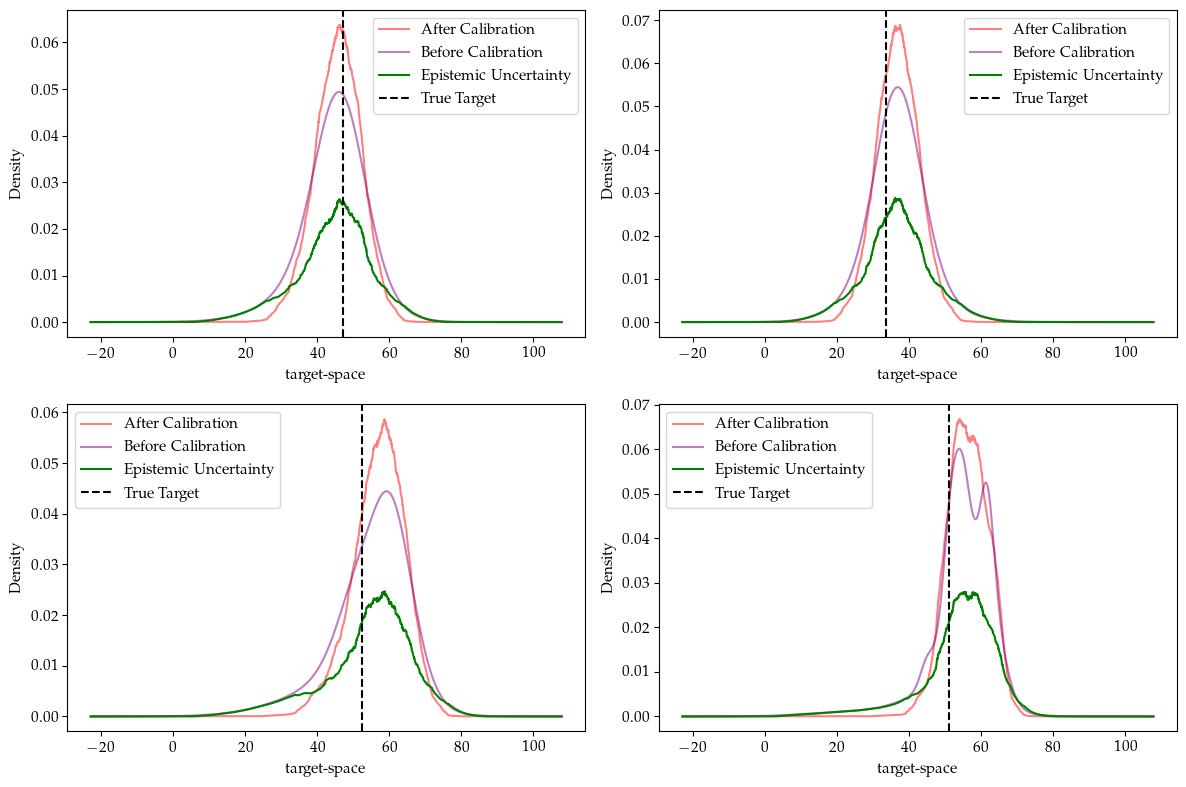
\includegraphics[width=0.8\textwidth]{resources/recalibration_concrete_dataset.png}
    \caption[Recalibration of the whole estimated conditional PDF]{Recalibration of the whole estimated conditional PDF on the Concrete dataset for four test samples. Calibrated on the train dataset and evaluated on the test dataset.}\label{fig:recalibration_concrete}
\end{figure}

Moreover, we can observe that recalibration of the full CDE can empirically compensate for a significant amount of model misspecification. In particular, as we can also see in \fef{fig:recalibration_grid} where the model was specified as an unimodal gaussian distribution but the true distribution is multimodal. In this case the recalibration can compensate for the misspecification as can even recover the bimodal distribution which makes it more than just a nice utility but a powerful tool that can be used to compensate and potentially identify model misspecification.

\subsubsection{Limitations of the Recalibration}

The recalibration of the whole CDE comes with certain limitations. Firstly, fully reconstructing the actual PDF requires extremely dense quantile and PDF grids. We used a PDF grid of up to $4096$ and a quantile grid of up to $256$. When considering the computational complexity behind the recalibration procedure this is already a significant amount of computation. Furthermore, another major limitation is that with a limited number of calibration samples the recalibration can actually overfit on the calibration samples. This is also part of why we empirically found that using the training samples for recalibration can increase the performance. Moreover, the recalibration can be very noisy and thus we need to smooth the recalibrated PDFs which necessarily introduces loss of information. Finally, finding the correct smoothing window is a non-trivial task and can significantly impact the performance of the recalibration.

We however believe that the recalibration of the whole CDE is a very powerful tool that can be used to compensate for model misspecification and can be used to identify model misspecification. Moreover, it can be used to obtain a quantification of the epistemic uncertainty of the model as we have shown in \pef{sec:uncertainty_calibration}. A deeper analysis of this method is left for future work.

\subsection{More Restriction on the possibly PDFs has a Regulatory Effect}\label{sec:experiment_results_more_restriction}

We claim that making stronger restrictions on $\mathscr{P}_\theta$ has a regulatory effect. In particular, we tested this on a toy dataset with a bimodal Gaussian distribution where we measured the performance as the error between the estimated $q = 0.25$ quantile and the true value, that we analytically know because it is a toy dataset. Two different approaches were used, a sparse approach where we only did MQR on three quantiles including the quantile of interest and a dense approach where we did MQR on $511$ quantiles. The quantiles were evenly spread between $0$ and $1$. On $50$ different samples of train and test set we observed that while the dense approach did not always outperform the sparse one it was more stable in terms of the variance and on average had a lower error. This is a strong indication that the hypothosized regulatory effect is present and that it can be used to improve the performance of the models. In \fef{fig:toy_dense_sparse} we can also observe this effect.

\begin{figure}
    \centering
    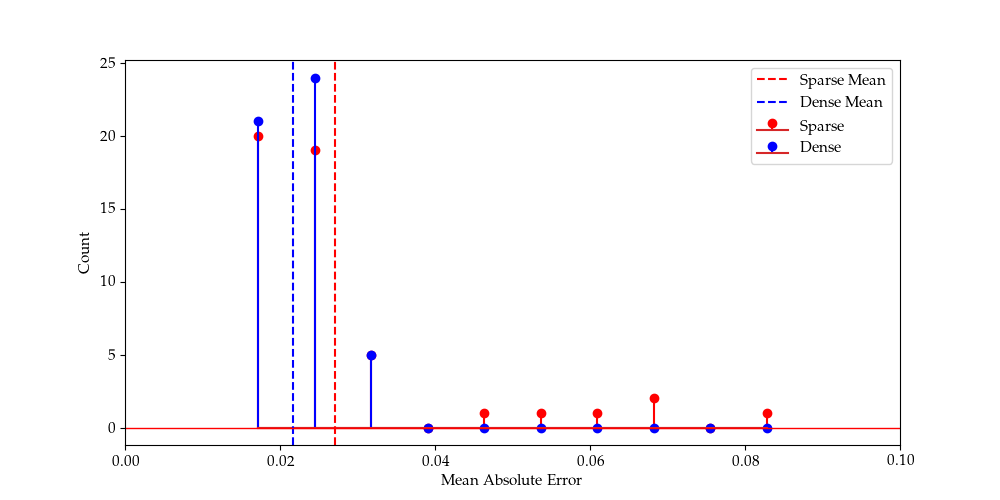
\includegraphics[width=0.8\textwidth]{resources/mean_absolute_error.png}
    \caption[Histogram of Dense vs. Sparse Quantile Restriction]{Histogram of Dense vs. Sparse Quantile Restriction. We can observe that the dense approach is more stable and on average over $50$ runs has a lower error.}\label{fig:toy_dense_sparse}
\end{figure}

\subsection{Main Benchmark Results}
Here we show the results of the final experiments on the 12 datasets in \tef{tab:results_interval_size_hdr} and \tef{tab:results_interval_size_hdr_connected}. The main experimental procedure, as can be seen in \sref[Algorithm]{alg:evaluation}, consisted for each dataset except for the two Voest ones of five-fold nested cross validation to obtain a robust estimate of the actual performance. On the two Voest Datasets instead we decided to always use the same train-test split where we consider the time dependence in the data by using the chronologically first 80\% of the data as training data and the last 20\% as test data. For the other datasets we used 80\%-20\% train-test spilts which is notably different from~\cite{sesia2021conformal} who used a fixed test set of 2000 samples, 2000 for calibration and the other part for training. In particular, on all datasets that we have the same, we have signlificantly less train dat but still competitive results.  Moreover, we do cross-validation on a time series split where we expand the training data and use the chronolocially last part for validation. This algorithm inspired by~\cite{rothfuss2019noise} is a nested cross validation algorithm over multiple seeds and hyperparameters that gurantees a robust estimate of the performance of the models on the test set. In particular, the test set is only used for the final evaluation and the hyperparameters are tuned on the training set which we do CV on.

\begin{algorithm}
    \caption{Evaluation of the Models}\label{alg:evaluation}
    \begin{algorithmic}
        \STATE\textbf{Input:} Hyperparameter Grid $H$, Model Class $M$, Dataset $D$, Number of Folds $K$, Number of Nested Folds $L$
        \STATE\textbf{Output:} Performance Metrics $P$

        \FOR{$k$ in $1, \dots, K$}
        \STATE$D_{\text{train}, k}, D_{\text{test}, k} \leftarrow \text{split}(D, k)$

        \STATE$CVSplits \leftarrow \text{split}(D_{\text{train}, k}, L)$

        \FOR{$h$ in $H$}
        \FOR{$D'_{\text{train}} D'_{\text{val}}$ in $CVSplits$}
        \STATE$M_h \leftarrow \text{fit}(M, D'_{\text{train}}, h)$
        \STATE$P_h \leftarrow \text{score}(M_h, D'_{\text{val}})$
        \ENDFOR%
        \ENDFOR%

        \STATE$h_{\text{best}} \leftarrow H[\text{argmax}(P)]$ Also set calibrated hyperparameters like epoch and $\alpha$ for CP

        \STATE$P_k \leftarrow \text{fit}(M, D_{\text{train}}, h_{\text{best}})$
        \STATE$P_k \leftarrow \text{score}(M_k, D_{\text{test}})$
        \ENDFOR%

        \STATE$P \leftarrow \text{mean}(P)$

        \RETURN$P$
    \end{algorithmic}
\end{algorithm}

\begin{table}[h!]
    \centering
    \caption[CDE Experiment Result CP with HDR Interval Size]{CDE Experiment Result CP with HDR Interval Size (lower is better)}\label{tab:results_interval_size_hdr}
    \begin{tabular}{l*{3}{d{3.8}}}
        \toprule
        \multicolumn{1}{c}{Dataset} & \multicolumn{1}{c}{MDN} & \multicolumn{1}{c}{KMN} & \multicolumn{1}{c}{MQR} \\
        \midrule
        Voest Realistic             & 198.59 \pm6.25          & 199.14 \pm4.91          & 198.85 \pm6.84          \\
        Voest Ideal                 & 117.48 \pm2.81          & 118.05 \pm3.08          & 118.52 \pm1.67          \\
        Boston Housing              & 9.45 \pm0.70            & 9.79 \pm0.35            & 9.32 \pm0.37            \\
        Concrete                    & 19.72 \pm0.71           & 19.37 \pm0.97           & 17.56 \pm0.55           \\
        Energy                      & 6.26 \pm0.18            & 3.99 \pm0.28            & 3.89 \pm0.27            \\
        CASP                        & 8.41 \pm0.17            & 7.81 \pm0.15            & 9.47 \pm0.18            \\
        Blog                        & 11.96 \pm0.76           & 11.83 \pm0.72           & 12.46 \pm0.77           \\
        Facebook 1                  & 12.19 \pm0.64           & 11.33 \pm0.64           & 11.34 \pm0.53           \\
        Facebook 2                  & 12.81 \pm1.72           & 12.02 \pm1.69           & 12.18 \pm1.55           \\
        Meps 19                     & 19.41 \pm1.59           & 19.49 \pm1.22           & 21.13 \pm1.22           \\
        Meps 20                     & 19.26 \pm1.00           & 18.53 \pm0.96           & 19.98 \pm0.89           \\
        Meps 21                     & 19.02 \pm1.17           & 18.85 \pm0.87           & 20.65 \pm0.78           \\
        \bottomrule
    \end{tabular}
\end{table}

\begin{table}[h!]
    \centering
    \caption[CDE Experiment Result CP with HDR Connected Interval Size]{CDE Experiment Result CP with HDR Connected Interval Size (lower is better)}\label{tab:results_interval_size_hdr_connected}
    \begin{tabular}{l*{3}{d{3.8}}}
        \toprule
        \multicolumn{1}{c}{Dataset} & \multicolumn{1}{c}{MDN} & \multicolumn{1}{c}{KMN} & \multicolumn{1}{c}{MQR} \\
        \midrule
        Voest Realistic             & 199.90 \pm5.93          & 210.30 \pm5.51          & 200.56 \pm7.27          \\
        Voest Ideal                 & 117.99 \pm2.83          & 136.04 \pm3.60          & 120.16 \pm1.87          \\
        Boston Housing              & 9.60 \pm0.77            & 10.23 \pm0.55           & 9.32 \pm0.37            \\
        Concrete                    & 19.88 \pm0.72           & 19.39 \pm0.96           & 17.56 \pm0.55           \\
        Energy                      & 6.53 \pm0.23            & 4.22 \pm0.29            & 3.89 \pm0.27            \\
        CASP                        & 11.29 \pm0.26           & 11.05 \pm0.20           & 10.27 \pm0.26           \\
        Blog                        & 12.12 \pm0.77           & 17.89 \pm1.33           & 15.57 \pm1.43           \\
        Facebook 1                  & 12.27 \pm0.64           & 15.81 \pm1.31           & 13.21 \pm0.93           \\
        Facebook 2                  & 12.84 \pm1.71           & 15.22 \pm1.62           & 13.78 \pm1.85           \\
        Meps 19                     & 19.86 \pm1.66           & 29.67 \pm2.40           & 22.90 \pm1.59           \\
        Meps 20                     & 19.59 \pm1.15           & 27.32 \pm2.28           & 21.34 \pm1.14           \\
        Meps 21                     & 19.75 \pm1.46           & 28.31 \pm1.72           & 22.37 \pm1.14           \\
        \bottomrule
    \end{tabular}
\end{table}

\subsection{Computational Complexity and Runtime}
Training CDM type models in our cases is per single training run not very computationally expensive. In particular, the NN architecture as described in \pef{sec:base_architecture} is for todays standards not of high complexity. However, since we decided to provide rigourous results by utilizing nested CV as in \sref[Algorithm]{alg:evaluation} the computational complexity increases significantly. However, still we consider the required computational resources to be very reasonable. All experiments could be done in about two weeks including all the first and second stage experiments which in total, when considering the separate training runs, are around 150000 runs as a rough estimate. However, we observed that on some datasets the training time can be significantly longer. In particular, CASP dataset took by far the longest since it only stopped early after more than 200 epochs sometimes while other datasets stopped already after ten epochs. We suggest for future studies in the paradigm of CDM to use the  CASP datset since it is appears to involve also multimodalities which can be very challenging for certain models. In particular this suspicion can be observed by comparing the results in \tef{tab:results_interval_size_hdr} and \tef{tab:results_interval_size_hdr_connected} where the connected intervals are significantly larger on the CASP dataset.

\subsection{Discussion}\label{sec:discussion}
As expected, resuls in the table with connected intervals are only slightly larger than the true HDR region sizes. Comparing our results to the current SOTA which is~\cite{sesia2021conformal} to our best knowledge, we can see that on many benchmarks we beat the results with pure HDR and even in some instances like the CASP dataset when using connected intervals which proofs that our methods and hyperparameters are very competitive. There is currently to the best of our knowledge no other work that applies CP to the Concrete, Boston Housing or Energy datasets, so we can not compare our results to other works. Specifically, there is actually a result for the Concrete dataset in~\cite{romano2019conformalized}, but they used an odd normalization techique where they divided the targets by the mean absolute target. Moreover, the instance of the concrete datasets used are non-identical which is why we do not bring a direct comparison. We used the concrete dataset in the work of~\cite{rothfuss2019noise}.

\subsubsection{Statistically Significant Results}
In order to test the statistical significance of our results we compare our best results with results from~\cite{sesia2021conformal} by utilizing Welch's t-test~\cite{welch1947generalization}.

The best results generally we obtain on the CASP dataset. Even for connected HDR intervals we outperform~\cite{sesia2021conformal} with a P-value of $0.034$. Moreover, for Meps 19 and Meps 21 we outperform the current NN implementation with a P-value of $0123213.045$ and $0.01232312148$ respectively. For the other datasets we obtain slightly worse results, but still very competitive.

When looking at the disconnected HDR regions, we dominate even more on the CASP dataset. In particular, we outperform the current SOTA with a P-value of $0$. We suspect that the CASP dataset has some major multimodalities which our model can capture very well. On the Meps datsets we also outperform the current SOTA when using HDR regions. However, on the other datasets we are still competitive but do not outperform the current SOTA.\@

\subsubsection{Why do we not always outperform the current SOTA?}

As we also used the same architecture MQR as~\cite{sesia2021conformal} we suspect that the partial worse performance is due to the hyperparameters that we used, but as the scope of this work is not to do a hyperparameter search we did not investigate this further. Moreover, it is noteworthy that we write our performance scores with a smaller train set as~\cite{sesia2021conformal}.

\subsubsection{Voest Dataset Discussion}

For the Voest Datasets we attempted multiple different model-approaches, including methods like the long-short term memory (LSTM) and gated recurrent unit (GRU). However, empirically the results actually worsened when adding information from this time-dimension. In the end we decided to use the same architecture as for the other datasets. The results are shown in \tef{tab:results_interval_size_hdr} and \tef{tab:results_interval_size_hdr_connected}.

Moreover, in \fef{fig:voest_ideal_test_set} we visualize a part of the dataset and the prediction on it for the Voest Ideal dataset in September 2023 with a 97\% confidence region. It can be observed that the model captures the time-dependencies in the data well. We suspect that the main bottleneck for the performance of the models on the Voest datasets is the information encoded in the features. In particular, in \tef{tab:results_interval_size_hdr} we can see that by using the ideal features we can already very significantly improve the performance, which of course is of limited practical use. However, it seems reasonable to believe that with more sophisticated feature engineering and more data sources the performance could be improved further also in a realistic setting.

\begin{figure}
    \centering
    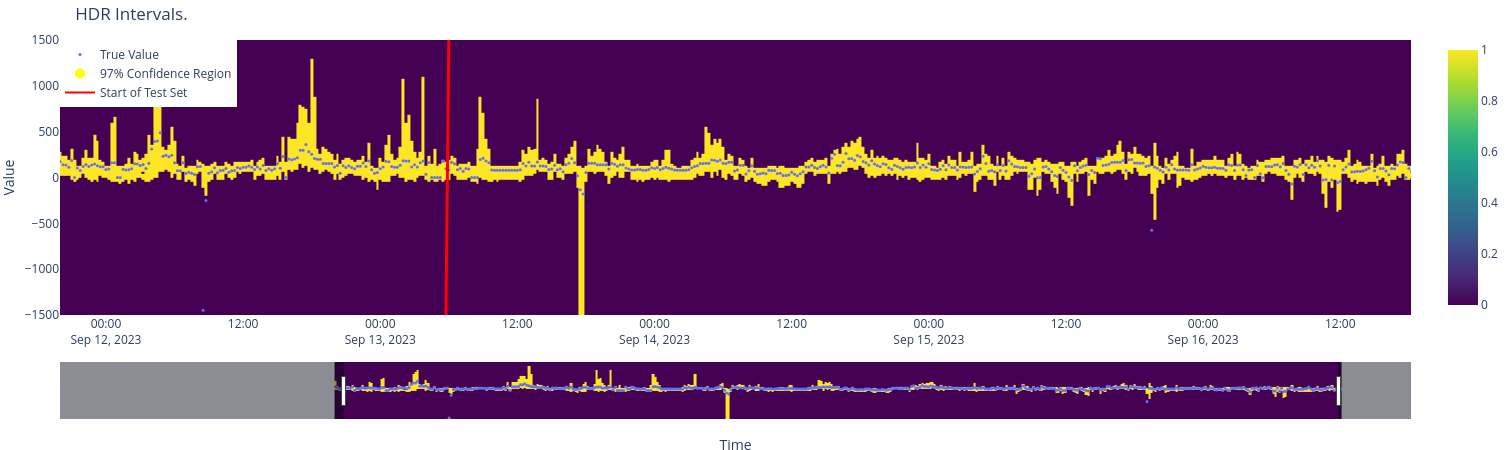
\includegraphics[width=1\textwidth]{resources/voest_ideal_test_set.png}
    \caption[Visualization of the Timeseries in Ideal Voest]{Visualization of the Timeseries in Ideal Voest during Sepember 2023. We can observe certain time-dependencies in the data.}\label{fig:voest_ideal_test_set}
\end{figure}

\chapter{Conclusion}\label{chap:conclusion}

In this work, we set out to unify the theory of CDE, QR, and CP under a common framework of CDM in which we are restricting the set of possible conditional probability density functions $\mathscr{P}_\theta$. Through rigorous theoretical analysis, we showed that these seemingly distinct tasks can be viewed as different approaches to the same underlying goal.

Building upon our theoretical foundation, we proposed using HDR to identify optimal conformal regions and introduced recalibration techniques to quantify epistemic uncertainty in CDE models. These methodological innovations were extensively validated through empirical studies on a diverse set of 12 datasets. Our methods consistently achieved strong performance, with SOTA results on several key benchmarks like the CASP dataset with statistical significance.

By enabling more accurate and reliable uncertainty quantification, our CDMs can support better decision making in consequential applications such as healthcare, where patient outcomes are at stake, and finance, where expensive investments depend on well-calibrated risk estimates. In particular, our work not only provides SOTA results but actually the interpretability of our results are the main strength, which is competely novel. We hope that this framework will allow certain applications to be more transparent and interpretable.

\section{Future Work}
There are many opportunities for future work in the field of CDMs. However, most importantly we believe a more thorough investigation of the recalibration of the whole CDE is necessary. In particular, we believe that the recalibration can be used to identify model misspecification and can be used to compensate for it. Moreover, we believe that the recalibration can be used to quantify the epistemic uncertainty of the model. A more thorough investigation of this method is left for future work. Secondly, a study that focuses on the effect of non-IID data, like for time-series data, in the context of CDM and the framework of restricted conditional PDFs is necessary.


%%%%%%%%%%%%%%%%%%
\printbibliography

%%%%%%%%%
\appendix

\end{document}